\documentclass[krantz2]{krantz}\usepackage{knitr}

\usepackage{color}

\usepackage{hologo}

\usepackage{csquotes}

\usepackage{graphicx}
\DeclareGraphicsExtensions{.jpg,.pdf,.png}

\usepackage{animate}

\usepackage[style=authoryear-comp,giveninits,sortcites,maxcitenames=2,%
    mincitenames=1,maxbibnames=10,minbibnames=10,backref,uniquename=mininit,%
    uniquelist=minyear,sortgiveninits=true,backend=biber]{biblatex}

\newcommand{\href}[2]{\emph{#2} (\url{#1})}

\usepackage{framed}

\usepackage{abbrev}
\usepackage{usingr}

\usepackage{imakeidx}

% this is to reduce spacing above and below verbatim, which is used by knitr
% to show returned values
\usepackage{etoolbox}
\makeatletter
\preto{\@verbatim}{\topsep=-5pt \partopsep=-4pt \itemsep=-2pt}
\makeatother

% for drawing flowcharts
\usepackage{tikz}
\usetikzlibrary{shapes.geometric,positioning,fit,arrows}
\tikzstyle{startstop} = [rectangle, rounded corners, minimum width=3cm, minimum height=1cm,text centered, draw=black]
\tikzstyle{io} = [trapezium, trapezium left angle=70, trapezium right angle=110, minimum width=3cm, minimum height=1cm, text centered, draw=black]
\tikzstyle{process} = [rectangle, minimum width=3cm, minimum height=1cm, text centered, draw=black]
%tight boxes
\tikzstyle{tprocess} = [rectangle, minimum width=2cm, minimum height=0.66cm, text centered, draw=black]
\tikzstyle{enclosure} = [rectangle, minimum width=3.4cm, minimum height=3cm, text centered, draw=black]
\tikzstyle{decision} = [diamond, aspect=2, minimum width=3cm, minimum height=1cm, text centered, draw=black]
\tikzstyle{arrow} = [thick,->,>=latex]

\tikzset{
 a/.style
  = {node distance=4em, text width=0.1em, minimum height=4em},
 b/.style
  = {rectangle, draw, fill=gray!10, node distance=4em, text width=6em,
     text centered, rounded corners, minimum height=4em, thick},
 c/.style
  = {circle, draw, dashed, fill=orange!10, inner sep = 0pt, node distance=4em, text width=6em,
     text centered, thick},
 cc/.style
  = {circle, draw, dashed, fill=orange!10, inner sep = 0pt, node distance=4em, text width=3em,
     text centered, thick},
 l/.style
  = {draw, -latex, ultra thick},
 aa/.style
  = {node distance=4em, text width=0em, minimum height=0.5ex},
 ll/.style
  = {draw, {open triangle 45} -, thick},
}

%\usepackage{polyglossia}
%\setdefaultlanguage{english}

\setcounter{topnumber}{3}
\setcounter{bottomnumber}{3}
\setcounter{totalnumber}{4}
\renewcommand{\topfraction}{0.90}
\renewcommand{\bottomfraction}{0.90}
\renewcommand{\textfraction}{0.10}
\renewcommand{\floatpagefraction}{0.70}
\renewcommand{\dbltopfraction}{0.90}
\renewcommand{\dblfloatpagefraction}{0.70}

% ensure page numbers are aligned in TOC
\makeatletter
\renewcommand{\@pnumwidth}{2.05em}
\makeatother

\addbibresource{rbooks.bib}
\addbibresource{references.bib}

\makeindex[title=General index]
\makeindex[name=rindex,title=Alphabetic index of \Rlang names]
\makeindex[name=rcatsidx,title=Index of \Rlang names by category]
\makeindex[name=cloudindex]
\IfFileExists{upquote.sty}{\usepackage{upquote}}{}
\begin{document}
\hyphenation{pro-cess-ing paren-the-ses spe-cif-ic au-thors in-ter-act-ed lim-it}

\title{\Huge{\fontseries{ub}\sffamily Learn R\\{\Large As a Language}}}

\author{Pedro J. Aphalo}

\date{Helsinki, \today}

% knitr setup

















\frontmatter

\maketitle

\newpage

\setcounter{page}{5} %previous pages will be reserved for frontmatter to be added in later.
\tableofcontents
\listoffigures



%\include{frontmatter/foreword}
%\chapter*{Preface}

\begin{VF}
``Suppose that you want to teach the `cat' concept to a very young child. Do you explain that a cat is a relatively small, primarily carnivorous mammal with retractible claws, a distinctive sonic output, etc.? I'll bet not. You probably show the kid a lot of different cats, saying `kitty' each time, until it gets the idea. To put it more generally, generalizations are best made by abstraction from experience.''

\VA{R. P. Boas}{Can we make mathematics intelligible?}
\end{VF}

%\dictum[R. P. Boas (1981) Can we make mathematics intelligible?, \emph{American Mathematical Monthly} \textbf{88:} 727-731.]{"Suppose that you want to teach the `cat' concept to a very young child. Do you explain that a cat is a relatively small, primarily carnivorous mammal with retractible claws, a distinctive sonic output, etc.? I'll bet not. You probably show the kid a lot of different cats, saying `kitty' each time, until it gets the idea. To put it more generally, generalizations are best made by abstraction from experience."}


% Such pauses are not a miss use of our time. To learn a natural language we need to interact with other speakers, we need feedback. In the case of R, we can get feedback both from the outcomes from our utterances to the computer, and from other \Rlang users.}
\noindent
This book covers different aspects of the use of the \Rlang language. Chapters \ref{chap:R:introduction} to \ref{chap:R:functions} describe the \Rlang language itself. Later chapters describe extensions to the \Rlang language available through contributed \emph{packages}, the \emph{grammar of data} and the \emph{grammar of graphics}. In this book, explanations are concise but contain pointers to additional sources of information, so as to encourage the development of a routine of independent exploration. This is not an arbitrary decision, this is the normal \emph{modus operandi} of most of us who use \Rlang regularly for a variety of different problems. Some have called approaches like the one used here ``learning the hard way'', but I would call it ``learning to be independent''.

I do not discuss statistics or data analysis methods in this book, I describe \Rlang as a language for data manipulation and display. The idea is for you to learn the \Rlang language in a way comparable to how children learn a language: they work out what the rules are, simply by listening to people speak and trying to utter what they want to tell their parents. Of course, small children receive some guidance, but they are not taught a prescriptive set of rules like when learning a second language at school. Instead of listening, you will read code and instead of speaking you will try to execute \Rlang  code statements on a computer---i.e. you will try your hand at using \Rlang to tell a computer what you want it to compute. I do provide explanations and guidance, but the idea of this book is for you to use the numerous examples to find out by yourself the overall patterns and coding philosophy behind the \Rlang language. Instead of parents being the sound board for your first utterances in \Rlang, the computer will play this role. You will \emph{play} by modifying the examples, see how the computer responds: does \Rlang understand you or not? Using a language actively is the most efficient way of learning it. By using it, I mean actually reading, writing and running scripts or programs (copying and pasting, or typing ready-made examples from books or the internet does not qualify as using a language).

I have been using \Rlang since around 1998 or 1999, but I am still constantly learning new things about \Rlang itself and \Rlang packages. With time it has replaced in my work as a researcher and teacher several other pieces of software: \pgrmnameNI{SPSS}, \pgrmnameNI{Systat}, \pgrmnameNI{Origin}, \pgrmnameNI{MS-Excel}, and it has become a central piece of the tool set I use for producing lecture slides, notes, books and even web pages. This is to say that it is the most useful piece of software and programming language I have ever learnt to use. Of course, in time it will be replaced by something better, but at the moment it is a key language to learn for anybody with a need to analyse and display data.

What is a language? A language is a system of communication. \Rlang as a language allows us to communicate with other members of the \Rlang community, and with computers. As all languages in active use, \Rlang evolves. New ``words'' and new ``constructs'' are incorporated into the language, and some earlier frequently used ones are relegated to the fringes of the corpus. I describe current usage and ``modisms'' of the \Rlang language in a way accessible to a readership unfamiliar with computer science but with some background in data analysis as used in Biology, Engineering, or Humanities.

When teaching I tend to lean towards challenging students rather than telling an over-simplified story. There are two reasons for this. First, I prefer as a student, and I learn best myself if the going is not too easy. Second, if I would hide the tricky bits of the \Rlang language, it would make readers' life much more difficult later on. You will not remember all the details, nobody could. However, you most likely will remember or develop a sense of in which situations you need to be careful or should check the details. So, I will expose you not only the usual cases, but also to several exceptions and counterintuitive features of the language, which I have highlighted with icons. Reading this book will be about exploring a new world; this book aims to be a travel guide, but neither a traveler's account, nor a cookbook of \Rlang recipes.

Keep in mind that it is impossible to remember everything about \Rlang! The \Rlang language in a broad sense is vast because its capabilities can be expanded with independently developed packages. Learning to use \Rlang consists in learning the basics plus developing the skill of finding your way in \Rlang and its documentation.  In 2017 the number packages available in the Comprehensive \Rlang Archive Network (CRAN) broke the 10\,000 barrier. CRAN is the most important, but not only, public repository for \Rlang packages. How good a command of the \Rlang language and packages a user needs depends on the type of activities to be carried out. This book attempts to train you in the use of the \Rlang language itself and of popular \Rlang language extensions for data manipulation and graphical display. Given the availability of numerous books on statistical analysis with \Rlang, in the present book I will cover only the bare minimum of this subject. The same is true for package development in \Rlang. This book seats in-between, aiming at teaching programming in-the-small: the use of \Rlang to automate the drudgery of data manipulation from raw data, through data exploration to the production of publication quality illustrations.

As with all ``rich'' languages there are many different ways of doing things in \Rlang, and there is in almost all cases no one-size-fits-all solution to a problem. There is always a compromise involved, usually between time spent by the user and processing time required in the computer. Many of the packages that are most popular nowadays did not exist when I started using \Rlang, and many of these packages make new approaches available. One could write many different \Rlang books with a given aim using substantially different ways of achieving the same results. In this book, I limit myself to packages that are currently popular and/or that I consider elegantly designed. I have in particular tried to limit myself to packages with similar design philosophies, especially in relation to their interfaces. What is elegant design, and in particular what is a friendly user interface depends strongly on each user's preferences and previous experience. Consequently, the contents of the book are strongly biased by my own preferences. I have tried to write examples in ways that execute fast without compromising readability. I encourage readers to take this book as a starting point for exploring the very many packages, styles and approaches which I have not described.

I will appreciate suggestions for further examples, notification of errors and unclear sections. Many of the examples here have been collected from diverse sources over many years and because of this not all sources are acknowledged. If you recognize any example as yours or someone else's please let me know so that I can add a proper acknowledgement. I warmly thank the students that over the years have asked the questions and posed the problems that have helped me write this text and correct the mistakes and voids of previous versions. I have also received help on on-line forums and in person from numerous people, learnt from archived e-mail list messages, blog posts, books, articles, tutorials, webinars, and by struggling to solve some new problems on my own. In many ways this text owes much more to people who are not authors than to myself. However, as I am the one who has written this version and decided what to include and exclude, as author, I take full responsibility for any errors and inaccuracies.

Why have I chosen the title ``\emph{Learn R \ldots as you learnt your mother tongue}''? On one hand, because this book is based on exploration and practice. On the other hand, because you will be exposed to current usage and not spared the quirks of the language. When we use our mother tongue in everyday life we do not think about grammar rules or sentence structure, except for the trickier or unfamiliar situations. My aim is for this book to help you grow to use \Rlang in this same way, to become fluent in \Rlang. The book is structured around the elements of languages with chapter titles that highlight the parallels between natural languages like English and the \Rlang language.

\emph{I encourage you to approach \Rlang, like a child approaches his or hers mother tongue when first learning to speak: Do not struggle, just play, fool around with \Rlang! If going gets difficult and frustrating, take a break! If you get a new insight, take a break to enjoy the victory!
}%\end{framed}

\newpage
%\vfill
%\begin{framed}
\noindent
\section*{Icons used to mark different content}

Text boxes are used throughout the book to highlight content that plays specific roles in the learning process or that require special attention from the reader. Each box contains one of five different icons that indicate the type of its contents as described below.\\[1.5ex]

\noindent
\playicon\ Signals \emph{playground} boxes which contain open-ended exercises---ideas and pieces of \Rlang code to play with at the \Rlang console.\\[1.5ex]

\noindent
\advplayicon\ Signals \emph{advanced playground} which will require more time to play with before grasping concepts than regular \emph{playground} boxes.\\[1.5ex]

\noindent
\ilAttention\ Signals important bits of information that must be remembered when using \Rlang---i.e.\ explain some unusual feature of the language.\\[1.5ex]

\noindent
\ilAdvanced\ Signals in-depth explanations of specific points that may require you to spend time thinking, which en general can be skipped on first reading, but to which you should return at a later, peaceful, time preferably with a cup of coffee or tea.\\[1.5ex]

\noindent
\infoicon\ Signals text boxes providing general information not directly related to the \Rlang language.\\[1.5ex]
%\end{framed}
%\newpage

%\newpage
%\begin{infobox}
%\noindent
%\textbf{Status as of 2016-11-23.} I have updated the manuscript to track package updates since the previous version uploaded six months ago, and added several examples of the new functionality added to packages \ggpmisc, \ggrepel, and \ggplot. I have written new sections on packages \viridis, \pkgname{gganimate}, \pkgname{ggstance}, \pkgname{ggbiplot}, \pkgname{ggforce}, \pkgname{ggtern} and \pkgname{ggalt}. Some of these sections are to be expanded, and additional sections are planned for other recently released packages.
%
%With respect to the chapter \textit{Storing and manipulating data with R} I have put it on hold, except for the introduction, until I can see a soon to be published book covering the same subject. Hadley Wickham has named the set of tools developed by him and his collaborators as \textit{tidyverse} to be described in the book titled \textit{R for Data Science} by Grolemund and Wickham (O'Reilly).
%
%An important update to \ggplot was released last week, and it includes changes to the behavior of some existing functions, specially faceting has become extensible through other packages. Several of the new facilities are described in the updated text and code included in this book and this pdf has been generated with up-to-date version of \ggplot and packages as available today from CRAN, except for \pkgname{ggtern} which was downloaded from Bitbucket minutes ago.
%
%The present update adds about 100 pages to the previous versions. I expect to upload a new update to this manuscript in one or two months time.
%
%\textbf{Status as of 2017-01-17.} Added ``playground'' exercises to the chapter describing \ggplot, and converted some of the examples earlier part of the main text into these playground items. Added icons to help readers quickly distinguish playground sections (\textcolor{blue}{\noticestd{"0055}}), information sections (\textcolor{blue}{\modpicts{"003D}}), warnings about things one needs to be specially aware of (\colorbox{yellow}{\typicons{"E136}}) and boxes with more advanced content that may require longer time/more effort to grasp (\typicons{"E04E}). Added to the sections \code{scales} and examples in the \ggplot chapter details about the use of colors in \Rlang and \ggplot2. Removed some redundant examples, and updated the section on \code{plotmath}. Added terms to the alphabetical index. Increased line-spacing to avoid uneven spacing with inline code bits.
%
%\textbf{Status as of 2017-02-09.} Wrote section on ggplot2 themes, and on using system- and Google fonts in ggpplots with the help of package \pkgname{showtext}. Expanded section on \ggplot's \code{annotation}, and revised some sections in the ``R scripts and Programming'' chapter. Started writing the data chapter. Wrote draft on writing and reading text files. Several other smaller edits to text and a few new examples.
%
%\textbf{Status as of 2017-02-14.} Wrote sections on reading and writing MS-Excel files, files from statistical programs such as SPSS, SyStat, etc., and NetCDF files. Also wrote sections on using URLs to directly read data, and on reading HTML and XML files directly, as well on using JSON to retrieve measured/logged data from IoT (internet of things) and similar intelligent physical sensors, micro-controller boards and sensor hubs with network access.
%
%\textbf{Status as of 2017-03-25.} Revised and expanded the chapter on plotting maps, adding a section on the manipulation and plotting of image data. Revised and expanded the chapter on extensions to \pkgname{ggplot2}, so that there are no longer empty sections. Wrote short chapter ``If and when \Rlang needs help''. Revised and expanded the ``Introduction'' chapter. Added index entries, and additional citations to literature.
%
%\textbf{Status as of 2017-04-04.} Revised and expanded the chapter on using \Rpgrm as a calculator. Revised and expanded the ``Scripts'' chapter. Minor edits to ``Functions'' chapter. Continued writing chapter on data, writing a section on \Rlang native apply functions and added preliminary text for a pipes and tees section. Write intro to `tidyverse' and grammar of data manipulation. Added index entries, and a few additional citations to the literature. Spell checking.
%
%\textbf{Status as of 2017-04-08.} Completed writing first draft of chapter on data, writing all the previously missing sections on the ``grammar of data manipulation''. Wrote two extended examples in the same chapter. Add table listing several extensions to \pkgname{ggplot2} not described in the book.
%
%\textbf{Status as of 2017-04-13.} Revised all chapters correcting some spelling mistakes, adding some explanatory text and indexing all functions and operators used. Thoroughly revised the Introduction chapter and the Preface. Expanded section on bar plots (now bar and column plots). Revised section on tile plots. Expanded section on factors in chapter 2, adding examples of reordering of factor labels, and making clearer the difference between the labels of the levels and the levels themselves.
%
%\textbf{Status as of 2017-04-29.} Tested with R 3.4.0. Package \pkgname{gganimate} needs to be installed from Github as the updated version is not yet in CRAN. Function \code{gg\_animate()} has been renamed \code{gganimate().}
%
%\textbf{Status as of 2017-05-14.} Submitted package \pkgname{learnrbook} to CRAN. Revised code in the book
%to use this new package. Small fixes after more testing. Added examples of plotting and labeling based on fits with \code{method = "nls"}, including use of the new \code{ggpmisc::stat\_fit\_tidy()}.
%
%\textbf{Status as of 2017-06-11.} Added sections on R-code bench marking and profiling for performance optimization. Added also an example of explicit compilation of a function defined in the R language. Added section on functions \code{assign()}, \code{get()} and \code{mget()}.
%
%\textbf{Status as of 2017-08-12.} Various edits to all chapters. Expanded section on \pkgname{ggpmisc} to include the new functionality added in version 0.2.15.9002: \code{geom\_table} and \code{stat\_fit\_tb}. Added section on package \pkgname{ggbeeswarm}. Added sections on packages \pkgname{magick} and on using \pgrmname{ImageJ} from \Rpgrm. Improved indexing and cross references.
%
%\textbf{Status as of 2017-10-25.} Edited the chapter on using R as a calculator, adding examples on insertion and deletion of members of lists and vectors, and also of use of \code{gl()} and \code{reorder()}. Edited sections on scale limits and added new section on coordinate limits to explain more thoroughly their differences and uses in chapter on plotting with \pkgname{ggplot2}. Added a section on package \pkgname{ggsignif} to the chapter on extensions to \pkgname{ggplot2}. Expanded section on \pkgname{ggpmisc} in the same chapter describing new functionality added in version 0.2.16.
%\pkgname{ggplo2} $>=$ 2.2.1.9000 is required by the current development version of \pkgname{ggpmisc}.
%
%\textbf{Status as of 2017-10-30.}  Add section on using pipes with \code{ggplot()} and layers.
%\end{infobox} 



\mainmatter






% !Rnw root = appendix.main.Rnw



\chapter{The R language: ``Paragraphs'' and ``essays''}\label{chap:R:scripts}
\index{scripts}

\begin{VF}
An \Rlang script is simply a text file containing (almost) the same commands that you would enter on the command line of \Rlang.

\VA{Jim Lemon}{\emph{Kickstarting R}}\nocite{LemonND}
\end{VF}

%\dictum[\href{https://cran.r-project.org/doc/contrib/Lemon-kickstart/}{Kickstarting R}]{An R script is simply a text file containing (almost) the same commands that you would enter on the command line of R.}\vskip2ex

\section{Aims of this chapter}

For those who have mainly used graphical user interfaces, understanding why and when scripts can help in communicating a certain data analysis protocol can be revelatory. As soon as a data analysis stops being trivial, describing the steps followed through a system of menus and dialogue boxes becomes extremely tedious.

Moreover, graphical user interfaces tend to be difficult to extend or improve in a way that keeps step-by-step instructions valid across program versions and operating systems.

Many times, exactly the same sequence of commands needs to be applied to different data sets, and scripts make both implementation and validation of such a requirement easy.

In this chapter, I will walk you through the use of \Rpgrm scripts, starting from an extremely simple script.

\section{Writing scripts}

In \Rlang language, the closest match to a natural language essay is a script. A script is built from multiple interconnected code statements needed to complete a given task. Simple statements can be combined into compound statements, which are the equivalent of natural language paragraphs. Scripts can vary from simple scripts containing only a few code statements, to complex scripts containing hundreds of code statements. In the rest of the present section I discuss how to write readable and reliable scripts and how to use them.

\subsection{What is a script?}\label{sec:script:what:is}
\index{scripts!definition}
A \textit{script} is a text file that contains (almost) the same commands that you would type at the console prompt. A true script is not, for example, an MS-Word file where you have pasted or typed some \Rlang commands.

When typing commands/statements at the \Rlang console, we "feed" one line of text at a time. When we end the line by typing the enter key, the line of text is interpreted and evaluated. We then type the next line of text, which gets in turn interpreted and evaluated, and so on. In a script we write nearly the same text in an editor and save multiple lines containing commands into a text file. Interpretation takes place only later, when we \emph{source} the file as a whole into \Rlang.

A script file has the following characteristics.
\begin{itemize}
  \item The script is a text file.
  \item The file contains valid \Rlang statements (including comments) and nothing else.
  \item Comments start at a \code{\#} and end at the end of the line.
  \item The \Rlang statements are in the file in the order that they must be executed.
  \item \Rlang scripts have file names ending in \texttt{.r} or \texttt{.R}.
\end{itemize}

The statements in the text file, are read, interpreted and evaluated sequentially, from the start to the end of the file, as represented in the diagram. We use \textcolor{blue}{$\cdots$} to represent additional statements in the script.

\begin{center}
\begin{small}
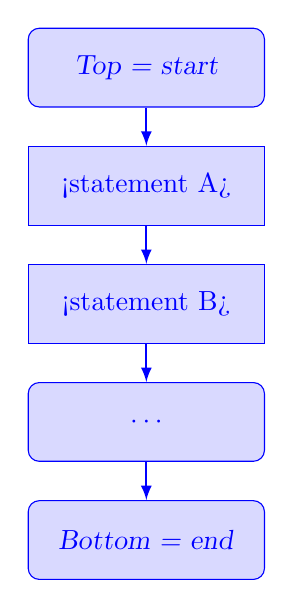
\begin{tikzpicture}[node distance=1.5cm]
\node (start) [startstop, color = blue, fill = blue!15] {\textsl{Top = start}};
\node (stat2) [process, color = blue, fill = blue!15, below of=start] {\code{<statement A>}};
\node (stat3) [process, color = blue, fill = blue!15, below of=stat2] {\code{<statement B>}};
\node (continue) [startstop, color = blue, fill = blue!15, below of=stat3] {$\cdots$};
\node (stop) [startstop, color = blue, fill = blue!15, below of=continue] {\textsl{Bottom = end}};
\draw [arrow, color = blue] (start) -- (stat2);
\draw [arrow, color = blue] (stat2) -- (stat3);
\draw [arrow, color = blue] (stat3) -- (continue);
\draw [arrow, color = blue] (continue) -- (stop);
\end{tikzpicture}
\end{small}
\end{center}

As we will see later in the chapter, code statements can be combined into larger statements and evaluated conditionally and/or repeatedly, which allows us to control the realised sequence of evaluated statements. Scripts need to respect the \Rlang syntax. In addition to being valid it is important that scripts are also understandable to humans, consequently a clear writing style and consistent adherence to it are important.

It is good practice to write scripts so that they are self-contained. To make a script self-contained, one must include calls to \texttt{library()} to load the packages used, load or import data from files, perform the data analysis and display and/or save the results of the analysis. Such scripts can be used to apply the same analysis algorithm to other data and/or to reproduce the same analysis at a later time. Such scripts document all steps used for the analysis.



\subsection{How do we use a script?}\label{sec:script:using}
\index{scripts!sourcing}

A script can be ``sourced'' using function \Rfunction{source()}. If we have a text file called \texttt{my.first.script.r} containing the following text:
\begin{shaded}
\footnotesize
\begin{verbatim}
# this is my first R script
print(3 + 4)
\end{verbatim}
\end{shaded}

and then source this file:

\begin{knitrout}\footnotesize
\definecolor{shadecolor}{rgb}{0.969, 0.969, 0.969}\color{fgcolor}\begin{kframe}
\begin{alltt}
\hlkwd{source}\hlstd{(}\hlstr{"my.first.script.r"}\hlstd{)}
\end{alltt}
\begin{verbatim}
## [1] 7
\end{verbatim}
\end{kframe}
\end{knitrout}

The results of executing the statements contained in the file will appear in the console. The commands themselves are not shown (by default the sourced file is not \emph{echoed} to the console) and the results will not be printed unless you include explicit \Rfunction{print()} commands in the script. This applies in many cases also to plots---e.g., a figure created with \Rfunction{ggplot()} needs to be printed if we want it to be included in the output when the script is run. Adding a redundant \Rfunction{print()} is harmless.

From within \RStudio, if you have an \Rpgrm script open in the editor, there will be a ``source'' icon visible with an attached drop-down menu from which you can choose ``Source'' as described above, or ``Source with echo,'' or ``Source as local job'' for the script in the currently active editor tab.

When a script is \emph{sourced}, the output can be saved to a text file instead of being shown in the console. It is also easy to call \Rpgrm with the \Rlang script file as an argument directly at the operating system shell or command-interpreter prompt---and obviously also from shell scripts. The next two chunks show commands entered at the OS shell command prompt rather than at the \Rlang command prompt.
\begin{shaded}
\footnotesize
\begin{verbatim}
> RScript my.first.script.r
\end{verbatim}
\end{shaded}

You can open an operating system's \emph{shell} from the Tools menu in \RStudio, to run this command. The output will be printed to the shell console. If you would like to save the output to a file, use redirection using the operating system's syntax.
\begin{shaded}
\footnotesize
\begin{verbatim}
> RScript my.first.script.r > my.output.txt
\end{verbatim}
\end{shaded}

Sourcing is very useful when the script is ready, however, while developing a script, or sometimes when testing things, one usually wants to run (or \emph{execute}) one or a few statements at a time. This can be done using the ``run'' button\footnote{If you use a different IDE or editor with an \Rlang mode, the details will vary, but a run command will be usually available.} after either positioning the cursor in the line to be executed, or selecting the text that one would like to run (the selected text can be part of a line, a whole line, or a group of lines, as long as it is syntactically valid). The key-shortcut Ctrl-Enter is equivalent to pressing the ``run'' button in \RStudio.

\subsection{How to write a script}\label{sec:script:writing}
\index{scripts!writing}

As with any type of writing, different approaches may be preferred by different \Rlang users. In general, the approach used, or mix of approaches, will also depend on how confident you are that the statements will work as expected---you already know the best approach vs.\ you are exploring different alternatives.
\begin{description}
\item[If one is very familiar with similar problems] One would just create a new text file and write the whole thing in the editor, and then test it. This is rather unusual.
\item[If one is moderately familiar with the problem] One would write the script as above, but testing it, step by step, as one is writing it. This is usually what I do.
\item[If one is mostly playing around] Then if one is using \RStudio, one can type statements at the console prompt. As you should know by now, everything you run at the console is saved to the ``History.'' In \RStudio, the History is displayed in its own pane, and in this pane one can select any previous statement(s) and by clicking on a single icon, copy and paste them to either the \Rlang console prompt, or the cursor position in the editor pane. In this way one can build a script by copying and pasting from the history to your script file, the bits that have worked as you wanted.
\end{description}

\begin{playground}
By now you should be familiar enough with \Rlang to be able to write your own script.
\begin{enumerate}
  \item Create a new \Rpgrm script (in \RStudio, from the File menu, ``+'' icon, or by typing ``Ctrl + Shift + N'').
  \item Save the file as \texttt{my.second.script.r}.
  \item Use the editor pane in \RStudio to type some \Rpgrm commands and comments.
  \item \emph{Run} individual commands.
  \item \emph{Source} the whole file.
\end{enumerate}
\end{playground}

\subsection{The need to be understandable to people}\label{sec:script:readability}
\index{scripts!readability}

When you write a script, it is either because you want to document what you have done or you want re-use the script at a later time. In either case, the script itself although still meaningful for the computer, could become very obscure to you, and even more to someone seeing it for the first time. This must be avoided by spending time and effort on the writing style.

How does one achieve an understandable script or program?
\begin{itemize}
  \item Avoid the unusual. People using a certain programming language tend to use some implicit or explicit rules of style---style includes \textit{indentation} of statements, \textit{capitalization} of variable and function names. As a minimum try to be consistent with yourself.
  \item Use meaningful names for variables, and any other object. What is meaningful depends on the context. Depending on common use, a single letter may be more meaningful than a long word. However self-explanatory names are usually better: e.g.,  using \code{n.rows} and \code{n.cols} is much clearer than using \code{n1} and \code{n2} when dealing with a matrix of data. Probably \code{number.of.rows} and \code{number.of.columns} would make the script verbose, and take longer to type without gaining anything in return.
  \item How to make the words visible in names: traditionally in \Rlang one would use dots to separate the words and use only lower case. Some years ago, it became possible to use underscores. The use of underscores is quite common nowadays because in some contexts it is ``safer'', as in some situations a dot may have a special meaning. What we call ``camel case'' is only infrequently used in \Rlang programming but is common in other languages like Pascal. An example of camel case is \code{NumCols}.
\end{itemize}

\begin{playground}
Here is an example of bad style in a script. Read \href{https://google.github.io/styleguide/Rguide.xml}{Google's R Style Guide}%\footnote{This is just an example, similar, but not exactly the same style as the style I use myself.}
, and edit the code in the chunk below so that it becomes easier to read.

\begin{knitrout}\footnotesize
\definecolor{shadecolor}{rgb}{0.969, 0.969, 0.969}\color{fgcolor}\begin{kframe}
\begin{alltt}
\hlstd{a} \hlkwb{<-} \hlnum{2} \hlcom{# height}
\hlstd{b} \hlkwb{<-} \hlnum{4} \hlcom{# length}
\hlstd{C} \hlkwb{<-}
    \hlstd{a} \hlopt{*}
\hlstd{b}
\hlstd{C} \hlkwb{->} \hlstd{variable}
      \hlkwd{print}\hlstd{(}
\hlstr{"area: "}\hlstd{, variable}
\hlstd{)}
\end{alltt}
\end{kframe}
\end{knitrout}
\end{playground}

The points discussed above already help a lot. However, one can go further in achieving the goal of human readability by interspersing explanations and code ``chunks'' and using all the facilities of typesetting, even of formatted maths formulas and equations, within the listing of the script. Furthermore, by including the results of the calculations and the code itself in a typeset report built automatically, we can ensure that the results are indeed the result of running the code shown. This greatly contributes to data analysis reproducibility, which is becoming a widespread requirement for any data analysis both in academia and in industry. It is possible not only to typeset whole books like this one, but also whole data-based web sites with these tools.

In the realm of programming, this approach is called literate programming\index{literate programming} and was first proposed by Donald Knuth \autocite{Knuth1984a} through his \pgrmname{WEB} system. In the case of \Rpgrm programming, the first support of literate programming was through \pkgname{Sweave}, which has been mostly superseded by \pkgname{knitr} \autocite{Xie2013}. This package supports the use of \langname{Markdown} or \LaTeX\index{Latex@\LaTeX}\ \autocite{Lamport1994} as the markup language for the textual contents and also formats and adds syntax highlighting to code chunks. \langname{Rmarkdown} is an extension to \langname{Markdown} that makes it easier to include \Rlang code in documents (see \url{http://rmarkdown.rstudio.com/}). It is the basis of \Rlang packages that support typesetting large and complex documents (\pkgname{bookdown}), web sites (\pkgname{blogdown}), package vignettes (\pkgname{pkgdown}) and slides for presentations \autocite{Xie2016,Xie2018}. The use of \pkgname{knitr} is very well integrated into the \RStudio IDE.

This is not strictly an \Rlang programming subject, as it concerns programming in any language. On the other hand, this is an incredibly important skill to learn, but well described in other books and web sites cited in the previous paragraph. This whole book, including figures, has been generated using \pkgname{knitr} and the source code for the book is available through Bitbucket at \url{https://bitbucket.org/aphalo/learnr-book}.

\subsection{Debugging scripts}\label{sec:script:debug}
\index{scripts!debugging}

The use of the word \emph{bug} to describe a problem in computer hardware and software started in 1946 when a real bug, more precisely a moth, got between the contacts of a relay in an electromechanical computer causing it to malfunction and Grace Hooper described the first computer \emph{bug}. The use of the term bug in engineering predates the use in computer science, and consequently, the first use of bug in computing caught on easily because it represented an earlier-used metaphor becoming real.

A suitable quotation from a letter written by Thomas Alva Edison 1878 \autocite[as given by][]{Hughes2004}:
\begin{quotation}
  It has been just so in all of my inventions. The first step is an intuition, and comes with a burst, then difficulties arise--this thing gives out and [it is] then that ``Bugs''--as such little faults and difficulties are called--show themselves and months of intense watching, study and labor are requisite before commercial success or failure is certainly reached.
\end{quotation}

The quoted paragraph above makes clear that only very exceptionally does any new design fully succeed. The same applies to \Rlang scripts as well as any other non-trivial piece of computer code. From this it logically follows that testing and de-bugging are fundamental steps in the development of \Rlang scripts and packages. Debugging, as an activity, is outside the scope of this book. However, clear programming style and good documentation are indispensable for efficient testing and reuse.

Even for scripts used for analyzing a single data set, we need to be confident that the algorithms and their implementation are valid, and able to return correct results. This is true both for scientific reports, expert data-based reports and any data analysis related to assessment of compliance with legislation or regulations. Of course, even in cases when we are not required to demonstrate validity, say for decision making purely internal to a private organization, we will still want to avoid costly mistakes.

The first step in producing reliable computer code is to accept that any code that we write needs to be tested and, if possible, validated. Another important step is to make sure that input is validated within the script and a suitable error produced for bad input (including valid input values falling outside the range that can be reliably handled by the script).

If during testing, or during normal use, a wrong value is returned by a calculation, or no value (e.g.,  the script crashes or triggers a fatal error), debugging consists in finding the cause of the problem. The cause can be either a mistake in the implementation of an algorithm, as well as in the algorithm itself. However, many apparent \emph{bugs} are caused by bad or missing handling of special cases like invalid input values, rounding errors, division by zero, etc., in which a program crashes instead of elegantly issuing a helpful error message.

Diagnosing the source of bugs is, in most cases, like detective work. One uses hunches based on common sense and experience to try to locate the lines of code causing the problem. One follows different \emph{leads} until the case is solved. In most cases, at the very bottom we rely on some sort of divide-and-conquer strategy. For example, we may check the value returned by intermediate calculations until we locate the earliest code statement producing a wrong value. Another common case is when some input values trigger a bug. In such cases it is frequently best to start by testing if different ``cases'' of input lead to errors/crashes or not. Boundary input values are usually the telltale ones: e.g.,  for numbers, zero, negative and positive values, very large values, very small values, missing values (\code{NA}), vectors of length zero (\code{numeric()}), etc.

\begin{warningbox}
  \textbf{Error messages} When debugging, keep in mind that in some cases a single bug can lead to a whole cascade of error messages. Do also keep in mind that typing mistakes, originating when code is entered through the keyboard, can wreak havock in a script: usually there is little correspondence between the number of error messages and the seriousness of the bug triggering them. When several errors are triggered, start by reading the error message printed first, as later errors can be an indirect consequence of earlier ones.
\end{warningbox}

There are special tools, called debuggers, available, and they help enormously. Debuggers allow one to step through the code, executing one statement at a time, and at each pause, allowing the user to inspect the objects present in the \Rlang environment and their values. It is even possible to execute additional statements, say, to modify the value of a variable, while execution is paused. An \Rlang debugger is available within \RStudio and also through the \Rlang console.

When writing your first scripts, you will manage perfectly well, and learn more by running the script one line at a time and when needed temporarily inserting \code{print()} statements to ``look'' at how the value of variables changes at each step. A debugger allows a lot more control, as one can ``step in'' and ``step out'' of function definitions, and set and unset break points where execution will stop, which is especially useful when developing \Rlang packages.

When reproducing the examples in this chapter, do keep this section in mind. In addition, if you get stuck trying to find the cause of a bug, do extend your search both to the most trivial of possible causes, and to the least likely ones (such as a bug in a package installed from CRAN or \Rlang itself). Of course, when suspecting a bug in code you have not written, it is wise to very carefully read the documentation, as the ``bug'' may be just in your understanding of what a certain piece of code is expected to do.  Also keep in mind that as discussed on page \pageref{sec:intro:net:help}, you will be able to find online already-answered questions to many of your likely problems and doubts. For example, Googling for the text of an error message is usually well rewarded.

\begin{warningbox}
When installing packages from other sources than CRAN (e.g.,  development versions from GitHub, Bitbucket or R-Forge, or in-house packages) there is no warranty that conflicts will not happen. Packages (and their versions) released through CRAN are regularly checked for inter-compatibility, while packages released through other channels are usually checked against only a few packages.

Conflicts among packages can easily arise, for example, when they use the same names for objects or functions. In addition, many packages use functions defined in packages in the \Rlang distribution itself or other independently developed packages by importing them. Updates to depended-upon packages can ``break'' (make non-functional) the dependent packages or parts of them. The rigorous testing by CRAN detects such problems in most cases when package revisions are submitted, forcing package maintainers to fix problems before distribution through CRAN is possible. However, if you use other repositories, I recommend that you make sure that revised (especially if under development) versions do work with your own script, before their use in ``production'' (important) data analyses.
\end{warningbox}


\section{Control of execution flow}\label{sec:script:flow:control}
\index{control of execution flow}
By default \Rlang statements in a script are evaluated (or executed) in the sequence they appear in the script \textit{listing} or text. We give the name \emph{control of execution constructs} to those special statements that allow us to alter this default sequence, by either skipping or repeatedly evaluating individual statements. The statements whose evaluation is controlled can be either simple or compound. Some of the control of execution flow statements, function like \emph{ON-OFF switches} for program statements. Others allow statements to be executed repeatedly while or until a condition is met, or until all members of a list or a vector are processed.

These \emph{control of execution constructs} can be also used at the \Rlang console, but it is usually awkward to do so as they can extend over several lines of text. In simple scripts, the \emph{flow of execution} can be fixed and linear from the first to the last statement in the script. \emph{Control of execution constructs} are a crucial part of most scripts. As we will see next, a compound statement can include multiple simple or nested compound statements.

\subsection{Compound statements}\label{sec:script:compound:statement}
\index{compound code statements}\index{simple code statements}

Individual statements can be grouped into \emph{compound statements} by enclosed them in curly braces. Conceptually is like putting several statements into a box that allows us to operate with them as an anonymous whole.

\begin{center}
\begin{small}
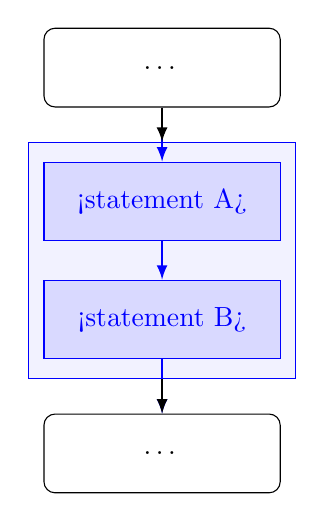
\begin{tikzpicture}[node distance=1.7cm]
\node (start) [startstop] {\ldots};
\node (enc) [enclosure, color = blue, fill = blue!5, below of=start, yshift=-0.75cm] {\ };
\node (stat2) [process, color = blue, fill = blue!15, below of=start] {\code{<statement A>}};
\node (stat3) [process, color = blue, fill = blue!15, below of=stat2, yshift=+0.2cm] {\code{<statement B>}};
\node (stop) [startstop, below of=stat3] {\ldots};
\draw [arrow, color = blue] (start) -- (stat2);
\draw [arrow, color = blue] (stat2) -- (stat3);
\draw [arrow, color = blue] (stat3) -- (stop);
\draw [arrow, color = black] (start) -- (enc);
\draw [arrow, color = black] (enc) -- (stop);
\end{tikzpicture}
\end{small}
\end{center}

\begin{knitrout}\footnotesize
\definecolor{shadecolor}{rgb}{0.969, 0.969, 0.969}\color{fgcolor}\begin{kframe}
\begin{alltt}
\hlkwd{print}\hlstd{(}\hlstr{"A"}\hlstd{)}
\end{alltt}
\begin{verbatim}
## [1] "A"
\end{verbatim}
\begin{alltt}
\hlstd{\{}
  \hlkwd{print}\hlstd{(}\hlstr{"B"}\hlstd{)}
  \hlkwd{print}\hlstd{(}\hlstr{"C"}\hlstd{)}
\hlstd{\}}
\end{alltt}
\begin{verbatim}
## [1] "B"
## [1] "C"
\end{verbatim}
\end{kframe}
\end{knitrout}

The grouping of the last two statements above is of no consequence by itself, but grouping becomes useful when used together with control-of-execution constructs.

\subsection{Conditional execution}
\index{conditional execution}

Conditional execution allows handling different values, such as negative and non-negative values, differently within a script. This is achieved by evaluating or not (i.e., switching ON and OFF) parts of a script based on the result returned by a logical expression. An \Rlang expression returning a logical value can be as simple as a logical value of \code{TRUE} or \code{FALSE} stored in a variable or the result of a computation done at the time of the flow-control decision.

\begin{explainbox}
We use the name \emph{flag} for a \code{logical} variable set manually, preferably near the top of the script. Use of flags is most useful when switching between two script behaviors depends on multiple sections of code. A frequent use case for flags is jointly enabling and disabling printing of output from multiple statements scattered in over a long script.
\end{explainbox}

\Rpgrm has two types of \emph{if}\index{conditional statements} statements, non-vectorized and vectorized. We will start with the non-vectorized one, which is similar to what is available in most other computer programming languages and controls the evaluation of a code statement, which can be either simple or compound.

\subsubsection[Non-vectorized \texttt{if}, \texttt{else} and \texttt{switch}]{Non-vectorized \code{if}, \code{else} and \code{switch}}
\qRcontrol{if()}\qRcontrol{if()\ldots else}%

The \code{if} construct ``decides,'' depending on a \code{logical} value, whether the next code statement is executed (if \code{TRUE}) or skipped (if \code{FALSE}). The flow chart shows how \code{if} works: \code{<statement A>} is either evaluated or skipped depending on the value of \code{<condition>}, while \code{<statement B>} is always evaluated.\label{flowchart:if}

\begin{center}
\begin{small}
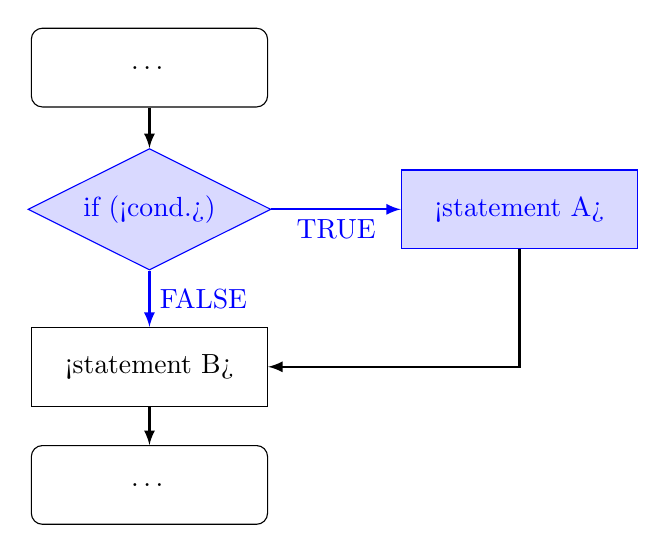
\begin{tikzpicture}[node distance=1.5cm]
\node (start) [startstop] {\ldots};
\node (dec1) [decision, color = blue, fill = blue!15, below of=start, yshift=-0.3cm] {\code{if (<cond.>)}};
\node (stat2) [process, color = blue, fill = blue!15, right of=dec1, xshift=3.2cm] {\code{<statement A>}};
\node (stat3) [process, below of=dec1, yshift=-0.5cm] {\code{<statement B>}};
\node (stop) [startstop, below of=stat3] {\ldots};
\draw [arrow] (start) -- (dec1);
\draw [arrow, color=blue] (dec1) -- node[anchor=north] {\code{TRUE}} (stat2);
\draw [arrow, color=blue] (dec1) -- node[anchor=west] {\code{FALSE}} (stat3);
\draw [arrow] (stat2) |- (stat3);
\draw [arrow] (stat3) -- (stop);
\end{tikzpicture}
\end{small}
\end{center}

We start with toy examples demonstrating how \emph{if} statements work. Later we will see examples closer to real use cases.

\begin{knitrout}\footnotesize
\definecolor{shadecolor}{rgb}{0.969, 0.969, 0.969}\color{fgcolor}\begin{kframe}
\begin{alltt}
\hlstd{flag} \hlkwb{<-} \hlnum{TRUE}
\hlkwa{if} \hlstd{(flag)} \hlkwd{print}\hlstd{(}\hlstr{"Hello!"}\hlstd{)}
\end{alltt}
\begin{verbatim}
## [1] "Hello!"
\end{verbatim}
\end{kframe}
\end{knitrout}

\begin{playground}
Play with the code above by changing the value assigned to variable \code{flag}, \code{FALSE}, \code{NA}, and \code{logical(0)}.

In the example above we use variable \code{flag} as the \emph{condition}.

Nothing in the \Rlang language prevents this condition from being a \code{logical} constant. Explain why \code{if (TRUE)} in the syntactically-correct statement below is of no practical use.

\begin{knitrout}\footnotesize
\definecolor{shadecolor}{rgb}{0.969, 0.969, 0.969}\color{fgcolor}\begin{kframe}
\begin{alltt}
\hlkwa{if} \hlstd{(}\hlnum{TRUE}\hlstd{)} \hlkwd{print}\hlstd{(}\hlstr{"Hello!"}\hlstd{)}
\end{alltt}
\begin{verbatim}
## [1] "Hello!"
\end{verbatim}
\end{kframe}
\end{knitrout}
\end{playground}

Conditional execution is much more useful than what could be expected from the previous example, because the statement whose execution is being controlled can be a compound statement of almost any length or complexity. A very simple example follows.

\begin{knitrout}\footnotesize
\definecolor{shadecolor}{rgb}{0.969, 0.969, 0.969}\color{fgcolor}\begin{kframe}
\begin{alltt}
\hlstd{printing} \hlkwb{<-} \hlnum{TRUE}
\hlkwa{if} \hlstd{(printing) \{}
  \hlkwd{print}\hlstd{(}\hlstr{"A"}\hlstd{)}
  \hlkwd{print}\hlstd{(}\hlstr{"B"}\hlstd{)}
\hlstd{\}}
\end{alltt}
\begin{verbatim}
## [1] "A"
## [1] "B"
\end{verbatim}
\end{kframe}
\end{knitrout}

\begin{warningbox}
The condition passed as an argument to \code{if}, enclosed in parentheses, can be anything yielding a \Rclass{logical} vector of length one. As this condition is \emph{not} vectorized, a longer vector will trigger an \Rlang warning or error depending on \Rlang's version.
\end{warningbox}

The \code{if \ldots\ else} construct ``decides,'' depending on a \code{logical} value, which of two code statements is executed. The flow chart shows how \code{if} works: either \code{<statement A>} or \code{<statement B>} is evaluated and the other skipped depending on the value of \code{<condition>}, while \code{<statement C>} is always evaluated.\label{flowchart:if:else}

\begin{center}
\begin{small}
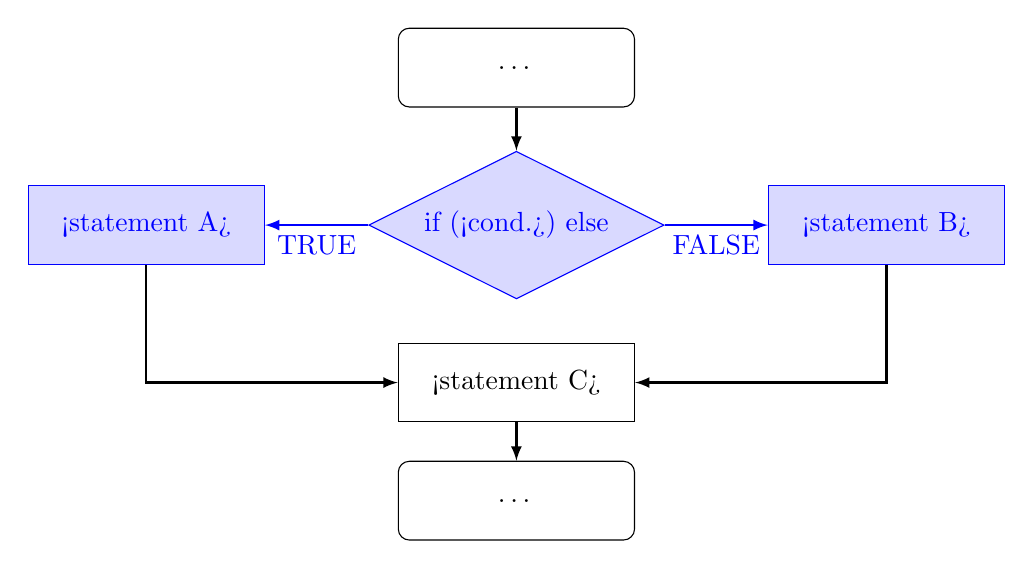
\begin{tikzpicture}[node distance=1.5cm]
\node (start) [startstop] {\ldots};
\node (dec1) [decision, color = blue, fill = blue!15, below of=start, yshift=-0.5cm] {\code{if (<cond.>) else}};
\node (stat2) [process, color = blue, fill = blue!15, left of=dec1, xshift=-3.2cm] {\code{<statement A>}};
\node (stat3) [process, color = blue, fill = blue!15, right of=dec1, xshift=3.2cm] {\code{<statement B>}};
\node (stat4) [process, below of=dec1, yshift=-0.5cm] {\code{<statement C>}};
\node (stop) [startstop, below of=stat4] {\ldots};
\draw [arrow] (start) -- (dec1);
\draw [arrow, color=blue] (dec1) -- node[anchor=north] {\code{TRUE}} (stat2);
\draw [arrow, color=blue] (dec1) -- node[anchor=north] {\code{FALSE}} (stat3);
\draw [arrow] (stat2) |- (stat4);
\draw [arrow] (stat3) |- (stat4);
\draw [arrow] (stat4) -- (stop);
\end{tikzpicture}
\end{small}
\end{center}

\begin{knitrout}\footnotesize
\definecolor{shadecolor}{rgb}{0.969, 0.969, 0.969}\color{fgcolor}\begin{kframe}
\begin{alltt}
\hlstd{a} \hlkwb{<-} \hlnum{10.0}
\hlkwa{if} \hlstd{(a} \hlopt{<} \hlnum{0.0}\hlstd{)} \hlkwd{print}\hlstd{(}\hlstr{"'a' is negative"}\hlstd{)} \hlkwa{else} \hlkwd{print}\hlstd{(}\hlstr{"'a' is not negative"}\hlstd{)}
\end{alltt}
\begin{verbatim}
## [1] "'a' is not negative"
\end{verbatim}
\begin{alltt}
\hlkwd{print}\hlstd{(}\hlstr{"This is always printed"}\hlstd{)}
\end{alltt}
\begin{verbatim}
## [1] "This is always printed"
\end{verbatim}
\end{kframe}
\end{knitrout}

As can be seen above, the statement immediately following \code{if} is executed if the condition returns \code{TRUE} and that following \code{else} is executed if the condition returns \code{FALSE}. Statements after the conditionally executed \code{if} and \code{else} statements are always executed, independently of the value returned by the condition.

\begin{playground}
Play with the code in the chunk above by assigning different numeric vectors to \code{a}.
\end{playground}



\begin{explainbox}
Do you still remember the rules about continuation lines?

\begin{knitrout}\footnotesize
\definecolor{shadecolor}{rgb}{0.969, 0.969, 0.969}\color{fgcolor}\begin{kframe}
\begin{alltt}
\hlcom{# 1}
\hlstd{a} \hlkwb{<-} \hlnum{1}
\hlkwa{if} \hlstd{(a} \hlopt{<} \hlnum{0.0}\hlstd{)} \hlkwd{print}\hlstd{(}\hlstr{"'a' is negative"}\hlstd{)} \hlkwa{else} \hlkwd{print}\hlstd{(}\hlstr{"'a' is not negative"}\hlstd{)}
\end{alltt}
\begin{verbatim}
## [1] "'a' is not negative"
\end{verbatim}
\end{kframe}
\end{knitrout}

Why does the statement below (not evaluated here) trigger an error while the one above does not?

\begin{knitrout}\footnotesize
\definecolor{shadecolor}{rgb}{0.969, 0.969, 0.969}\color{fgcolor}\begin{kframe}
\begin{alltt}
\hlcom{# 2 (not evaluated here)}
\hlkwd{if} (a < 0.0) \hlkwd{print}(\hlstr{"\hlstr{'a'} is negative"})
else \hlkwd{print}(\hlstr{"\hlstr{'a'} is not negative"})
\end{alltt}
\end{kframe}
\end{knitrout}

How do the continuation line rules apply when we add curly braces as shown below.

\begin{knitrout}\footnotesize
\definecolor{shadecolor}{rgb}{0.969, 0.969, 0.969}\color{fgcolor}\begin{kframe}
\begin{alltt}
\hlcom{# 1}
\hlstd{a} \hlkwb{<-} \hlnum{1}
\hlkwa{if} \hlstd{(a} \hlopt{<} \hlnum{0.0}\hlstd{) \{}
    \hlkwd{print}\hlstd{(}\hlstr{"'a' is negative"}\hlstd{)}
  \hlstd{\}} \hlkwa{else} \hlstd{\{}
    \hlkwd{print}\hlstd{(}\hlstr{"'a' is not negative"}\hlstd{)}
  \hlstd{\}}
\end{alltt}
\begin{verbatim}
## [1] "'a' is not negative"
\end{verbatim}
\end{kframe}
\end{knitrout}

In the example above, we enclosed a single statement between each pair of curly braces, but as these braces create compound statements, multiple statements could have been enclosed between each pair.
\end{explainbox}

\begin{playground}
Play with the use of conditional execution, with both simple and compound statements, and also think how to combine \code{if} and \code{else} to select among more than two options.
\end{playground}

In \Rlang, the value returned by any compound statement is the value returned by the last simple statement executed within the compound one. This means that we can assign the value returned by an \code{if} and \code{else} statement to a variable. This style is less frequently used, but occasionally can result in easier-to-understand scripts.\label{chunk:if:assignment}

\begin{knitrout}\footnotesize
\definecolor{shadecolor}{rgb}{0.969, 0.969, 0.969}\color{fgcolor}\begin{kframe}
\begin{alltt}
\hlstd{a} \hlkwb{<-} \hlnum{1}
\hlstd{my.message} \hlkwb{<-}
  \hlkwa{if} \hlstd{(a} \hlopt{<} \hlnum{0.0}\hlstd{)} \hlstr{"'a' is negative"} \hlkwa{else} \hlstr{"'a' is not negative"}
\hlkwd{print}\hlstd{(my.message)}
\end{alltt}
\begin{verbatim}
## [1] "'a' is not negative"
\end{verbatim}
\end{kframe}
\end{knitrout}

\begin{explainbox}
If the condition statement returns a value of a class other than \code{logical}, \Rlang will attempt to convert it into a logical. This is sometimes used instead of a comparison to zero, as the conversion from \code{integer} yields \code{TRUE} for all integers except zero. The code below illustrates a rather frequently used idiom for checking if there is something available to display.
\begin{knitrout}\footnotesize
\definecolor{shadecolor}{rgb}{0.969, 0.969, 0.969}\color{fgcolor}\begin{kframe}
\begin{alltt}
\hlstd{message} \hlkwb{<-} \hlstr{"abc"}
\hlkwa{if} \hlstd{(}\hlkwd{length}\hlstd{(message))} \hlkwd{print}\hlstd{(message)}
\end{alltt}
\begin{verbatim}
## [1] "abc"
\end{verbatim}
\end{kframe}
\end{knitrout}
\end{explainbox}

\begin{advplayground}
Study the conversion rules between \Rclass{numeric} and \Rclass{logical} values, run each of the statements below, and explain the output based on how type conversions are interpreted, remembering the difference between \emph{floating-point numbers} as implemented in computers and \emph{real numbers} ($\mathbb{R}$) as defined in mathematics.

% chunk contains intentional error-triggering examples
\begin{knitrout}\footnotesize
\definecolor{shadecolor}{rgb}{0.969, 0.969, 0.969}\color{fgcolor}\begin{kframe}
\begin{alltt}
\hlkwa{if} \hlstd{(}\hlnum{0}\hlstd{)} \hlkwd{print}\hlstd{(}\hlstr{"hello"}\hlstd{)}
\hlkwa{if} \hlstd{(}\hlopt{-}\hlnum{1}\hlstd{)} \hlkwd{print}\hlstd{(}\hlstr{"hello"}\hlstd{)}
\hlkwa{if} \hlstd{(}\hlnum{0.01}\hlstd{)} \hlkwd{print}\hlstd{(}\hlstr{"hello"}\hlstd{)}
\hlkwa{if} \hlstd{(}\hlnum{1e-300}\hlstd{)} \hlkwd{print}\hlstd{(}\hlstr{"hello"}\hlstd{)}
\hlkwa{if} \hlstd{(}\hlnum{1e-323}\hlstd{)} \hlkwd{print}\hlstd{(}\hlstr{"hello"}\hlstd{)}
\hlkwa{if} \hlstd{(}\hlnum{1e-324}\hlstd{)} \hlkwd{print}\hlstd{(}\hlstr{"hello"}\hlstd{)}
\hlkwa{if} \hlstd{(}\hlnum{1e-500}\hlstd{)} \hlkwd{print}\hlstd{(}\hlstr{"hello"}\hlstd{)}
\hlkwa{if} \hlstd{(}\hlkwd{as.logical}\hlstd{(}\hlstr{"true"}\hlstd{))} \hlkwd{print}\hlstd{(}\hlstr{"hello"}\hlstd{)}
\hlkwa{if} \hlstd{(}\hlkwd{as.logical}\hlstd{(}\hlkwd{as.numeric}\hlstd{(}\hlstr{"1"}\hlstd{)))} \hlkwd{print}\hlstd{(}\hlstr{"hello"}\hlstd{)}
\hlkwa{if} \hlstd{(}\hlkwd{as.logical}\hlstd{(}\hlstr{"1"}\hlstd{))} \hlkwd{print}\hlstd{(}\hlstr{"hello"}\hlstd{)}
\hlkwa{if} \hlstd{(}\hlstr{"1"}\hlstd{)} \hlkwd{print}\hlstd{(}\hlstr{"hello"}\hlstd{)}
\end{alltt}
\end{kframe}
\end{knitrout}

Hint: if you need to refresh your understanding of the type conversion rules, see section \ref{sec:calc:type:conversion} on page \pageref{sec:calc:type:conversion}.
\end{advplayground}

In addition to \Rcontrol{if ()} and \Rcontrol{if () \ldots\ else}, there is in \Rlang a \Rcontrol{switch()} statement, which we describe next. It can be used to select among \emph{cases}, or several alternative statements, based on an expression evaluating to a \code{numeric} or a \code{character} value of length equal to one. While \Rcontrol{if ()} and \code{if () \ldots\ else} allow for binary choices as they are controlled by a logical value, \Rcontrol{switch()} can control execution of many more statements. The usual way in which \Rcontrol{switch()} statement is used is by assignment of the returned value, as described as being rather unusual, but legal, for \code{if () \ldots\ else} on page \pageref{chunk:if:assignment}.

The switch statement returns a value, the value returned by the \Rcontrol{switch()} statement is that returned by the statement corresponding to the matching switch value, or the default (similar to \code{else}) if there is no match and a default return value has been defined. Each optional statement can be thought as a \textit{case} from a set of possible cases.\label{flowchart:switch}

\begin{center}
\begin{small}
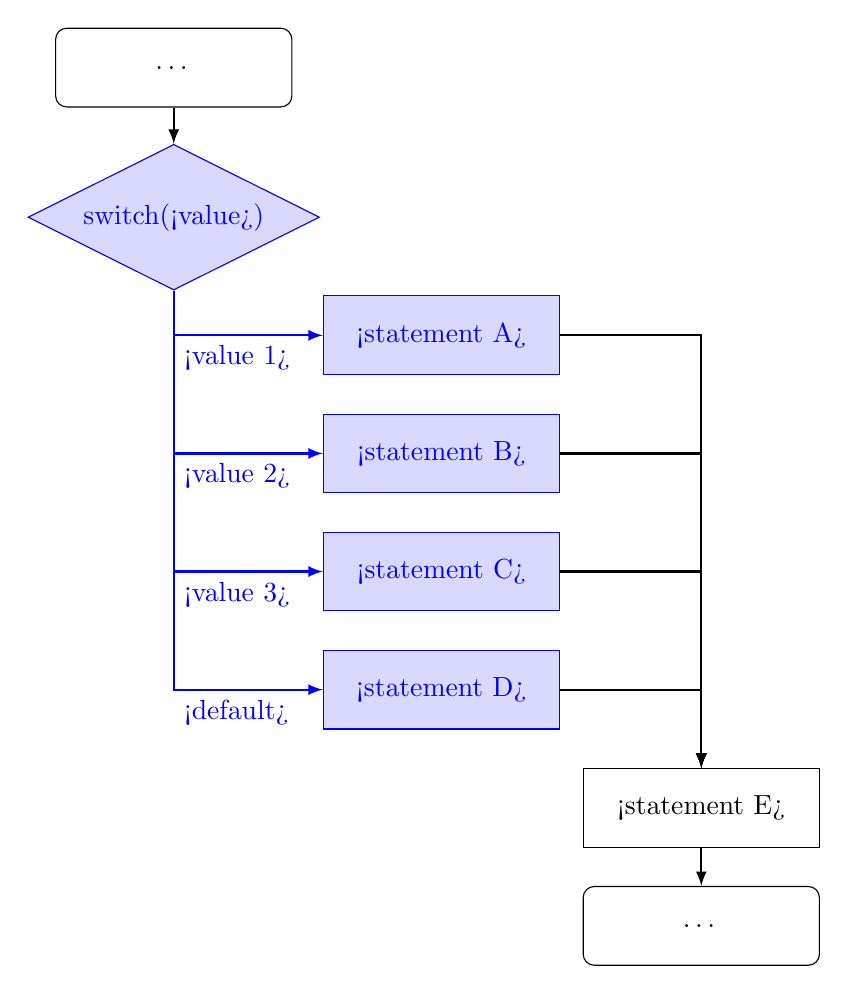
\begin{tikzpicture}[node distance=1.5cm]
\node (start) [startstop] {\ldots};
\node (dec1) [decision, color = blue, fill = blue!15, below of=start, yshift=-0.4cm] {\code{switch(<value>)}};
\node (stat2) [process, color = blue, fill = blue!15, below of=dec1, xshift=3.4cm] {\code{<statement A>}};
\node (stat3) [process, color = blue, fill = blue!15, below of=stat2] {\code{<statement B>}};
\node (stat4) [process, color = blue, fill = blue!15, below of=stat3] {\code{<statement C>}};
\node (stat5) [process, color = blue, fill = blue!15, below of=stat4] {\code{<statement D>}};
\node (stat6) [process, below of=stat5, xshift=3.3cm] {\code{<statement E>}};
\node (stop) [startstop, below of=stat6] {\ldots};
\draw [arrow] (start) -- (dec1);
\draw [arrow, color=blue] (dec1) |- node[anchor=north west] {\code{<value 1>}} (stat2);
\draw [arrow, color=blue] (dec1) |- node[anchor=north west] {\code{<value 2>}} (stat3);
\draw [arrow, color=blue] (dec1) |- node[anchor=north west] {\code{<value 3>}} (stat4);
\draw [arrow, color=blue] (dec1) |- node[anchor=north west] {\code{<default>}} (stat5);
\draw [arrow] (stat2) -| (stat6);
\draw [arrow] (stat3) -| (stat6);
\draw [arrow] (stat4) -| (stat6);
\draw [arrow] (stat5) -| (stat6);
\draw [arrow] (stat6) -- (stop);
\end{tikzpicture}
\end{small}
\end{center}

In the first example we use character constants saved in a variable as a condition, with the last statement with no tag being the default. Instead of the name of variable \code{my.object}, we could have used a complex expression returning a suitable \code{character} value of length one.

\begin{knitrout}\footnotesize
\definecolor{shadecolor}{rgb}{0.969, 0.969, 0.969}\color{fgcolor}\begin{kframe}
\begin{alltt}
\hlstd{my.object} \hlkwb{<-} \hlstr{"two"}
\hlstd{b} \hlkwb{<-} \hlkwd{switch}\hlstd{(my.object,}
            \hlkwc{one} \hlstd{=} \hlnum{1}\hlstd{,}
            \hlkwc{two} \hlstd{=} \hlnum{1} \hlopt{/} \hlnum{2}\hlstd{,}
            \hlkwc{four} \hlstd{=} \hlnum{1} \hlopt{/} \hlnum{4}\hlstd{,}
            \hlnum{0}
\hlstd{)}
\hlstd{b}
\end{alltt}
\begin{verbatim}
## [1] 0.5
\end{verbatim}
\end{kframe}
\end{knitrout}

Multiple condition values can share the same statement.

\begin{knitrout}\footnotesize
\definecolor{shadecolor}{rgb}{0.969, 0.969, 0.969}\color{fgcolor}\begin{kframe}
\begin{alltt}
\hlstd{my.object} \hlkwb{<-} \hlstr{"two"}
\hlstd{b} \hlkwb{<-} \hlkwd{switch}\hlstd{(my.object,}
            \hlkwc{one} \hlstd{=,} \hlkwc{uno} \hlstd{=} \hlnum{1}\hlstd{,}
            \hlkwc{two} \hlstd{=,} \hlkwc{dos} \hlstd{=} \hlnum{1} \hlopt{/} \hlnum{2}\hlstd{,}
            \hlkwc{four} \hlstd{=,} \hlkwc{cuatro} \hlstd{=} \hlnum{1} \hlopt{/} \hlnum{4}\hlstd{,}
            \hlnum{0}
\hlstd{)}
\hlstd{b}
\end{alltt}
\begin{verbatim}
## [1] 0.5
\end{verbatim}
\end{kframe}
\end{knitrout}
\begin{playground}
    Do play with the use of the switch statement. Look at the documentation for \code{switch()} using \code{help(switch)} and study the examples at the end of the help page. Explore what happens if you set \code{my.object <- "ten"}, \code{my.object <- "three"}, \code{my.object <- NA\_character\_} or  \code{my.object <- character()}. Then remove the \code{, 0} as default value, and repeat.
\end{playground}

When the expression used as a condition returns a value that is not a \code{character}, it will be interpreted as an \code{integer} index. In this case no names are used for the cases, and the last one is always interpreted as the default.

\begin{knitrout}\footnotesize
\definecolor{shadecolor}{rgb}{0.969, 0.969, 0.969}\color{fgcolor}\begin{kframe}
\begin{alltt}
\hlstd{my.number} \hlkwb{<-} \hlnum{2}
\hlstd{b} \hlkwb{<-} \hlkwd{switch}\hlstd{(my.number,}
            \hlnum{1}\hlstd{,}
            \hlnum{1} \hlopt{/} \hlnum{2}\hlstd{,}
            \hlnum{1} \hlopt{/} \hlnum{4}\hlstd{,}
            \hlnum{0}
\hlstd{)}
\hlstd{b}
\end{alltt}
\begin{verbatim}
## [1] 0.5
\end{verbatim}
\end{kframe}
\end{knitrout}

\begin{playground}
    Continue playing with the use of the switch statement. Explore what happens if you set \code{my.number <- 10}, \code{my.number <- 3}, \code{my.number <- NA} or  \code{my.object <- numeric()}. Then remove the \code{, 0} as default value, and repeat.
\end{playground}

\begin{explainbox}
The statements for the different values of the condition in a \Rcontrol{switch()} statement can be compound statements as in the case of \code{if}, and they can even be used for a side effect. We can for example modify the example above to print a message when the default value is returned.
\begin{knitrout}\footnotesize
\definecolor{shadecolor}{rgb}{0.969, 0.969, 0.969}\color{fgcolor}\begin{kframe}
\begin{alltt}
\hlstd{my.object} \hlkwb{<-} \hlstr{"ten"}
\hlstd{b} \hlkwb{<-} \hlkwd{switch}\hlstd{(my.object,}
            \hlkwc{one} \hlstd{=} \hlnum{1}\hlstd{,}
            \hlkwc{two} \hlstd{=} \hlnum{1} \hlopt{/} \hlnum{2}\hlstd{,}
            \hlkwc{three} \hlstd{=} \hlnum{1} \hlopt{/} \hlnum{4}\hlstd{,}
            \hlstd{\{}\hlkwd{print}\hlstd{(}\hlstr{"No match! Using default"}\hlstd{);} \hlnum{0}\hlstd{\}}
\hlstd{)}
\end{alltt}
\begin{verbatim}
## [1] "No match! Using default"
\end{verbatim}
\begin{alltt}
\hlstd{b}
\end{alltt}
\begin{verbatim}
## [1] 0
\end{verbatim}
\end{kframe}
\end{knitrout}
\end{explainbox}

\begin{explainbox}
  The \Rcontrol{switch()} statement can substitute for chained \code{if \ldots\ else} statements when all the conditions can be described by constant values or distinct values returned by the same test. The advantage is more concise and readable code. The equivalent of the first \Rcontrol{switch()} example above when written using \code{if \ldots\ else} becomes longer. Given how terse code using \Rcontrol{switch()} is, those not yet familiar with its use may find the more verbose style used below easier to understand. On the other hand, with numerous cases \Rcontrol{switch()} is easier to read and understand.

\begin{knitrout}\footnotesize
\definecolor{shadecolor}{rgb}{0.969, 0.969, 0.969}\color{fgcolor}\begin{kframe}
\begin{alltt}
\hlstd{my.object} \hlkwb{<-} \hlstr{"two"}
\hlkwa{if} \hlstd{(my.object} \hlopt{==} \hlstr{"one"}\hlstd{) \{}
  \hlstd{b} \hlkwb{<-} \hlnum{1}
\hlstd{\}} \hlkwa{else if} \hlstd{(my.object} \hlopt{==} \hlstr{"two"}\hlstd{) \{}
  \hlstd{b} \hlkwb{<-} \hlnum{1} \hlopt{/} \hlnum{2}
\hlstd{\}} \hlkwa{else if} \hlstd{(my.object} \hlopt{==} \hlstr{"four"}\hlstd{) \{}
  \hlstd{b} \hlkwb{<-} \hlnum{1} \hlopt{/} \hlnum{4}
\hlstd{\}} \hlkwa{else} \hlstd{\{}
  \hlstd{b} \hlkwb{<-} \hlnum{0}
\hlstd{\}}
\hlstd{b}
\end{alltt}
\begin{verbatim}
## [1] 0.5
\end{verbatim}
\end{kframe}
\end{knitrout}

\end{explainbox}

\subsubsection[Vectorized \texttt{ifelse()}]{Vectorized \code{ifelse()}}
\index{vectorized ifelse}
Vectorized \emph{ifelse} is a peculiarity of the \Rlang language, but very useful for writing concise code that may execute faster than logically equivalent but not vectorized code.
Vectorized conditional execution is coded by means of \emph{function} \Rcontrol{ifelse()} (written as a single word). This function takes three arguments: a \code{logical} vector usually the result of a test (parameter \code{test}), an expression to use for \code{TRUE} cases (parameter \code{yes}), and an expression to use for \code{FALSE} cases (parameter \code{no}). At each index position along the vectors, the value included in the returned vector is taken from \code{yes} if \code{test} is \code{TRUE} and from \code{no} if \code{test} is \code{FALSE}. All three arguments can be any \Rlang statement returning the required vectors. In the case of vectors passed as arguments to parameters \code{yes} and \code{no}, recycling will take place if they are shorter than the logical vector returned by the expression passed as argument to \code{test}. No recycling ever applies to \code{test}, even if \code{yes} and/or \code{no} are longer than \code{test}.

The flow chart for \Rcontrol{ifelse()} is similar to that for \code{if \ldots\ else} shown on page \pageref{flowchart:if} but applied in parallel to the individual members of vectors; e.g.\ the condition expression is evaluated at index position \code{1} controls which value will be present in the returned vector at index position \code{1}, and so on.

It is customary to pass arguments to \code{ifelse} by position. We give a first example with named arguments to clarify the use of the function.

\begin{knitrout}\footnotesize
\definecolor{shadecolor}{rgb}{0.969, 0.969, 0.969}\color{fgcolor}\begin{kframe}
\begin{alltt}
\hlstd{my.test} \hlkwb{<-} \hlkwd{c}\hlstd{(}\hlnum{TRUE}\hlstd{,} \hlnum{FALSE}\hlstd{,} \hlnum{TRUE}\hlstd{,} \hlnum{TRUE}\hlstd{)}
\hlkwd{ifelse}\hlstd{(}\hlkwc{test} \hlstd{= my.test,} \hlkwc{yes} \hlstd{=} \hlnum{1}\hlstd{,} \hlkwc{no} \hlstd{=} \hlopt{-}\hlnum{1}\hlstd{)}
\end{alltt}
\begin{verbatim}
## [1]  1 -1  1  1
\end{verbatim}
\end{kframe}
\end{knitrout}

In practice, the most common idiom is to have as an argument passed to \code{test}, the result of a comparison calculated on the fly. In the first example we compute the absolute values for a vector, equivalent to that returned by \Rlang function \code{abs()}.

\begin{knitrout}\footnotesize
\definecolor{shadecolor}{rgb}{0.969, 0.969, 0.969}\color{fgcolor}\begin{kframe}
\begin{alltt}
\hlstd{nums} \hlkwb{<-} \hlopt{-}\hlnum{3}\hlopt{:+}\hlnum{3}
\hlkwd{ifelse}\hlstd{(nums} \hlopt{<} \hlnum{0}\hlstd{,} \hlopt{-}\hlstd{nums, nums)}
\end{alltt}
\begin{verbatim}
## [1] 3 2 1 0 1 2 3
\end{verbatim}
\end{kframe}
\end{knitrout}

\begin{playground}
Some additional examples to play with, with a few surprises. Study the examples below until you understand why returned values are what they are. In addition, create your own examples to test other possible cases. In other words, play with the code until you fully understand how \code{ifelse} works.

\begin{knitrout}\footnotesize
\definecolor{shadecolor}{rgb}{0.969, 0.969, 0.969}\color{fgcolor}\begin{kframe}
\begin{alltt}
\hlstd{a} \hlkwb{<-} \hlnum{1}\hlopt{:}\hlnum{10}
\hlkwd{ifelse}\hlstd{(a} \hlopt{>} \hlnum{5}\hlstd{,} \hlnum{1}\hlstd{,} \hlopt{-}\hlnum{1}\hlstd{)}
\hlkwd{ifelse}\hlstd{(a} \hlopt{>} \hlnum{5}\hlstd{, a} \hlopt{+} \hlnum{1}\hlstd{, a} \hlopt{-} \hlnum{1}\hlstd{)}
\hlkwd{ifelse}\hlstd{(}\hlkwd{any}\hlstd{(a} \hlopt{>} \hlnum{5}\hlstd{), a} \hlopt{+} \hlnum{1}\hlstd{, a} \hlopt{-} \hlnum{1}\hlstd{)} \hlcom{# tricky}
\hlkwd{ifelse}\hlstd{(}\hlkwd{logical}\hlstd{(}\hlnum{0}\hlstd{), a} \hlopt{+} \hlnum{1}\hlstd{, a} \hlopt{-} \hlnum{1}\hlstd{)} \hlcom{# even more tricky}
\hlkwd{ifelse}\hlstd{(}\hlnum{NA}\hlstd{, a} \hlopt{+} \hlnum{1}\hlstd{, a} \hlopt{-} \hlnum{1}\hlstd{)} \hlcom{# as expected}
\end{alltt}
\end{kframe}
\end{knitrout}
Hint: if you need to refresh your understanding of \code{logical} values and Boolean algebra see section \ref{sec:calc:boolean} on page \pageref{sec:calc:boolean}.
\end{playground}

\begin{warningbox}
In the case of \Rcontrol{ifelse()}, the length of the returned value is determined by the length of the logical vector passed as an argument to its first formal parameter (named \code{test})! A frequent mistake is to use a condition that returns a \code{logical} vector of length one, expecting that it will be recycled because arguments passed to the other formal parameters (named \code{yes} and \code{no}) are longer. However, no recycling will take place, resulting in a returned value of length one, with the remaining elements of the vectors passed to \code{yes} and \code{no} being discarded. Do try this by yourself, using logical vectors of different lengths. You can start with the examples below, making sure you understand why the returned values are what they are.

\begin{knitrout}\footnotesize
\definecolor{shadecolor}{rgb}{0.969, 0.969, 0.969}\color{fgcolor}\begin{kframe}
\begin{alltt}
\hlkwd{ifelse}\hlstd{(}\hlnum{TRUE}\hlstd{,} \hlnum{1}\hlopt{:}\hlnum{5}\hlstd{,} \hlopt{-}\hlnum{5}\hlopt{:-}\hlnum{1}\hlstd{)}
\end{alltt}
\begin{verbatim}
## [1] 1
\end{verbatim}
\begin{alltt}
\hlkwd{ifelse}\hlstd{(}\hlnum{FALSE}\hlstd{,} \hlnum{1}\hlopt{:}\hlnum{5}\hlstd{,} \hlopt{-}\hlnum{5}\hlopt{:-}\hlnum{1}\hlstd{)}
\end{alltt}
\begin{verbatim}
## [1] -5
\end{verbatim}
\begin{alltt}
\hlkwd{ifelse}\hlstd{(}\hlkwd{c}\hlstd{(}\hlnum{TRUE}\hlstd{,} \hlnum{FALSE}\hlstd{),} \hlnum{1}\hlopt{:}\hlnum{5}\hlstd{,} \hlopt{-}\hlnum{5}\hlopt{:-}\hlnum{1}\hlstd{)}
\end{alltt}
\begin{verbatim}
## [1]  1 -4
\end{verbatim}
\begin{alltt}
\hlkwd{ifelse}\hlstd{(}\hlkwd{c}\hlstd{(}\hlnum{FALSE}\hlstd{,} \hlnum{TRUE}\hlstd{),} \hlnum{1}\hlopt{:}\hlnum{5}\hlstd{,} \hlopt{-}\hlnum{5}\hlopt{:-}\hlnum{1}\hlstd{)}
\end{alltt}
\begin{verbatim}
## [1] -5  2
\end{verbatim}
\begin{alltt}
\hlkwd{ifelse}\hlstd{(}\hlkwd{c}\hlstd{(}\hlnum{FALSE}\hlstd{,} \hlnum{TRUE}\hlstd{),} \hlnum{1}\hlopt{:}\hlnum{5}\hlstd{,} \hlnum{0}\hlstd{)}
\end{alltt}
\begin{verbatim}
## [1] 0 2
\end{verbatim}
\end{kframe}
\end{knitrout}
\end{warningbox}

\begin{playground}
Write, using \Rcontrol{ifelse()}, a single statement to combine numbers from the two vectors \code{a} and \code{b} into a result vector \code{d}, based on whether the corresponding value in vector \code{c} is the character \code{"a"} or \code{"b"}. Then print vector \code{d} to make the result visible.

\begin{knitrout}\footnotesize
\definecolor{shadecolor}{rgb}{0.969, 0.969, 0.969}\color{fgcolor}\begin{kframe}
\begin{alltt}
\hlstd{a} \hlkwb{<-} \hlopt{-}\hlnum{10}\hlopt{:-}\hlnum{1}
\hlstd{b} \hlkwb{<-} \hlopt{+}\hlnum{1}\hlopt{:}\hlnum{10}
\hlstd{c} \hlkwb{<-} \hlkwd{c}\hlstd{(}\hlkwd{rep}\hlstd{(}\hlstr{"a"}\hlstd{,} \hlnum{5}\hlstd{),} \hlkwd{rep}\hlstd{(}\hlstr{"b"}\hlstd{,} \hlnum{5}\hlstd{))}
\hlcom{# your code}
\end{alltt}
\end{kframe}
\end{knitrout}

If you do not understand how the three vectors are built, or you cannot guess the values they contain by reading the code, print them, and play with the arguments, until you understnd what each parameter does. Also use \code{help(rep)} and/or \code{help(ifelse)} to access the documentation.
\end{playground}

\subsection{Iteration}
\index{loops|seealso{iteration}}
We give the name \emph{iteration} to the process of repetitive execution of a program statement (simple or compound)---e.g., \emph{computed by iteration}. We use the same word, iteration, to name each one of these repetitions of the execution of a statement---e.g.,  the second iteration.

The section of computer code being executed multiple times, forms a loop (a closed path). Most loops contain a condition that determines when the flow of execution will exit the loop and continue at the next statement following the loop. In \Rlang three types of iteration loops are available: those using \Rloop{for}, \Rloop{while} and \Rloop{repeat} constructs. They differ in how much flexibility they provide with respect to the values they iterate over, and how the condition that terminates the iteration is tested. When the same algorithm can be implemented with more than one of these constructs, using the least flexible of them usually results in the easiest to understand \Rlang scripts. In \Rlang, rather frequently, explicit loops as described in this section can be replaced advantageously by calls to the \emph{apply} functions described in section \ref{sec:data:apply} on page \pageref{sec:data:apply}.

\subsubsection[\texttt{for} loops]{\code{for} loops}
The\index{for loop}\index{iteration!for loop}\qRloop{for} most frequently used type of loop is a \code{for} loop. These loops work in \Rlang on lists or vectors of values to act upon. The implicit test for the end of the vector or list takes place at the top of the construct before the loop statement is evaluated. The flow chart has a \emph{loop} as the execution can be directed to an earlier position in the sequence of statements, allowing the same code to be evaluated multiple times.

\begin{center}
\begin{small}
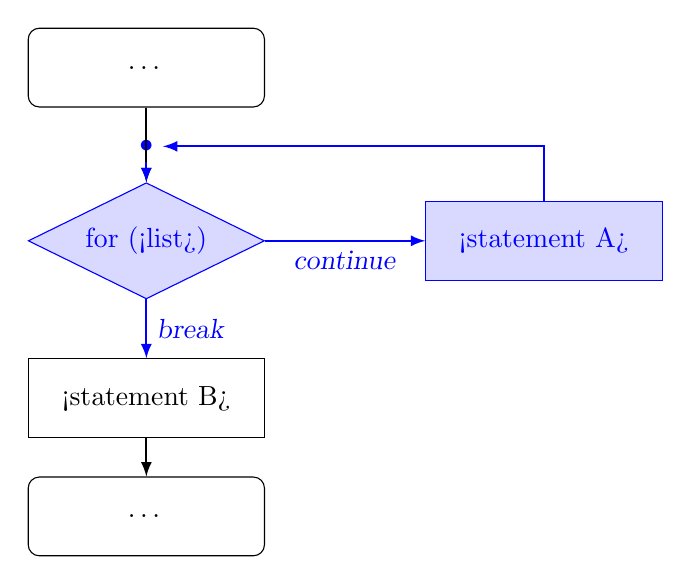
\begin{tikzpicture}[node distance=1.5cm]
\node (start) [startstop] {\ldots};
\node (entry) [below of=start, color = blue, yshift=0.5cm]{$\bullet$};
\node (dec1) [decision, color = blue, fill = blue!15, below of=entry, yshift=0.3cm] {\code{for (<list>)}};
\node (stat2) [process, color = blue, fill = blue!15, right of=dec1, xshift=3.55cm] {\code{<statement A>}};
\node (stat3) [process, below of=dec1, yshift=-0.5cm] {\code{<statement B>}};
\node (stop) [startstop, below of=stat3] {\ldots};
\draw [arrow] (start) -- (dec1);
\draw [arrow, color=blue] (dec1) -- node[anchor=north] {\textsl{continue}} (stat2);
\draw [arrow, color=blue] (dec1) -- node[anchor=west] {\textsl{break}} (stat3);
\draw [arrow, color = blue] (stat2) |- (entry);
\draw [arrow, color = blue] (entry) -- (dec1);
\draw [arrow] (stat3) -- (stop);
\end{tikzpicture}
\end{small}
\end{center}

\begin{knitrout}\footnotesize
\definecolor{shadecolor}{rgb}{0.969, 0.969, 0.969}\color{fgcolor}\begin{kframe}
\begin{alltt}
\hlstd{b} \hlkwb{<-} \hlnum{0}
\hlkwa{for} \hlstd{(a} \hlkwa{in} \hlnum{1}\hlopt{:}\hlnum{5}\hlstd{) b} \hlkwb{<-} \hlstd{b} \hlopt{+} \hlstd{a}
\hlstd{b}
\end{alltt}
\begin{verbatim}
## [1] 15
\end{verbatim}
\begin{alltt}
\hlstd{b} \hlkwb{<-} \hlkwd{sum}\hlstd{(}\hlnum{1}\hlopt{:}\hlnum{5}\hlstd{)} \hlcom{# built-in function (faster)}
\hlstd{b}
\end{alltt}
\begin{verbatim}
## [1] 15
\end{verbatim}
\end{kframe}
\end{knitrout}

Here the statement \code{b <- b + a} is executed five times, with variable \code{a} sequentially taking each of the values in \code{1:5}. Instead of a simple statement used here, a compound statement could also have been used for the body of the \Rloop{for} loop.

\begin{warningbox}
It is important to note that a list or vector of length zero is a valid argument to \code{for()}, that triggers no error, but skips the statements in the loop body.
\end{warningbox}

Some examples of use of \code{for} loops---and of how to avoid their use.

\begin{knitrout}\footnotesize
\definecolor{shadecolor}{rgb}{0.969, 0.969, 0.969}\color{fgcolor}\begin{kframe}
\begin{alltt}
\hlstd{a} \hlkwb{<-} \hlkwd{c}\hlstd{(}\hlnum{1}\hlstd{,} \hlnum{4}\hlstd{,} \hlnum{3}\hlstd{,} \hlnum{6}\hlstd{,} \hlnum{8}\hlstd{)}
\hlkwa{for}\hlstd{(x} \hlkwa{in} \hlstd{a) \{}\hlkwd{print}\hlstd{(x}\hlopt{*}\hlnum{2}\hlstd{)\}} \hlcom{# print is needed!}
\end{alltt}
\begin{verbatim}
## [1] 2
## [1] 8
## [1] 6
## [1] 12
## [1] 16
\end{verbatim}
\end{kframe}
\end{knitrout}

A call to \Rloop{for} does not return a value. We need to assign values to an object so that they are not lost. If we print at each iteration the value of this object, we can follow how the stored value changes. Printing allows us to see, how the vector grows in length, unless we create a long-enough vector before the start of the loop.

\begin{knitrout}\footnotesize
\definecolor{shadecolor}{rgb}{0.969, 0.969, 0.969}\color{fgcolor}\begin{kframe}
\begin{alltt}
\hlstd{b} \hlkwb{<-} \hlkwa{for}\hlstd{(x} \hlkwa{in} \hlstd{a) \{x}\hlopt{*}\hlnum{2}\hlstd{\}}
\hlstd{b}
\end{alltt}
\begin{verbatim}
## NULL
\end{verbatim}
\begin{alltt}
\hlstd{b} \hlkwb{<-} \hlkwd{numeric}\hlstd{()}
\hlkwa{for}\hlstd{(i} \hlkwa{in} \hlkwd{seq}\hlstd{(}\hlkwc{along.with} \hlstd{= a)) \{}
  \hlstd{b[i]} \hlkwb{<-} \hlstd{a[i]}\hlopt{^}\hlnum{2}
  \hlkwd{print}\hlstd{(b)}
\hlstd{\}}
\end{alltt}
\begin{verbatim}
## [1] 1
## [1]  1 16
## [1]  1 16  9
## [1]  1 16  9 36
## [1]  1 16  9 36 64
\end{verbatim}
\begin{alltt}
\hlstd{b}
\end{alltt}
\begin{verbatim}
## [1]  1 16  9 36 64
\end{verbatim}
\begin{alltt}
\hlcom{# runs faster if we first allocate a long enough vector}
\hlstd{b} \hlkwb{<-} \hlkwd{numeric}\hlstd{(}\hlkwd{length}\hlstd{(a))}
\hlkwa{for}\hlstd{(i} \hlkwa{in} \hlkwd{seq}\hlstd{(}\hlkwc{along.with} \hlstd{= a)) \{}
  \hlstd{b[i]} \hlkwb{<-} \hlstd{a[i]}\hlopt{^}\hlnum{2}
  \hlkwd{print}\hlstd{(b)}
\hlstd{\}}
\end{alltt}
\begin{verbatim}
## [1] 1 0 0 0 0
## [1]  1 16  0  0  0
## [1]  1 16  9  0  0
## [1]  1 16  9 36  0
## [1]  1 16  9 36 64
\end{verbatim}
\begin{alltt}
\hlstd{b}
\end{alltt}
\begin{verbatim}
## [1]  1 16  9 36 64
\end{verbatim}
\begin{alltt}
\hlcom{# a vectorized expression is simplest and fastest}
\hlstd{b} \hlkwb{<-} \hlstd{a}\hlopt{^}\hlnum{2}
\hlstd{b}
\end{alltt}
\begin{verbatim}
## [1]  1 16  9 36 64
\end{verbatim}
\end{kframe}
\end{knitrout}

In the previous chunk we used \code{seq(along.with = a)} to build a new numeric vector with a sequence of the same length as vector \code{a}. Using this \emph{idiom} is best as it ensures that even the case when \code{a} is an \emph{empty} vector of length zero will be handled correctly, with \code{numeric(0)} assigned to \code{b}.

\begin{playground}\label{box:play:forloop}
Look at the results from the above examples, and try to understand where the returned value comes from in each case. In the code chunk above, \Rfunction{print()} is used within the \emph{loop} to make intermediate values visible. You can add additional \code{print()} statements to visualize other variables, such as \code{i}, or run parts of the code, such as \code{seq(along.with = a)}, by themselves.

In this case, the code examples trigger no errors or warnings, but the same approach can be used for debugging syntactically correct code that does not return the expected results.
\end{playground}

\begin{advplayground}
In the examples above we show the use of \code{seq()} passing a vector as an argument to its parameter \code{along.with}. Run the examples below and explain why the two approaches are equivalent only when the length of \code{a} is one or more. Find the answer by assigning to \code{a}, vectors of different lengths, including zero (using \code{a <- numeric(0)}).

\begin{knitrout}\footnotesize
\definecolor{shadecolor}{rgb}{0.969, 0.969, 0.969}\color{fgcolor}\begin{kframe}
\begin{alltt}
\hlstd{b} \hlkwb{<-} \hlkwd{numeric}\hlstd{(}\hlkwd{length}\hlstd{(a))}
\hlkwa{for}\hlstd{(i} \hlkwa{in} \hlkwd{seq}\hlstd{(}\hlkwc{along.with} \hlstd{= a)) \{}
  \hlstd{b[i]} \hlkwb{<-} \hlstd{a[i]}\hlopt{^}\hlnum{2}
\hlstd{\}}
\hlkwd{print}\hlstd{(b)}

\hlstd{c} \hlkwb{<-} \hlkwd{numeric}\hlstd{(}\hlkwd{length}\hlstd{(a))}
\hlkwa{for}\hlstd{(i} \hlkwa{in} \hlnum{1}\hlopt{:}\hlkwd{length}\hlstd{(a)) \{}
  \hlstd{c[i]} \hlkwb{<-} \hlstd{a[i]}\hlopt{^}\hlnum{2}
\hlstd{\}}
\hlkwd{print}\hlstd{(c)}
\end{alltt}
\end{kframe}
\end{knitrout}

\end{advplayground}

\begin{explainbox}
\Rloop{for} loops as described above, in the absence of errors, have statically predictable behavior. The compound statement in the loop will be executed once for each member of the vector or list. Special cases may require the alteration of the normal flow of execution in the loop. Two cases are easy to deal with, one is stopping iteration early, which we can do with \Rloop{break()}, and another is jumping ahead to the start of the next iteration, which we can do with \Rloop{next()}.
\end{explainbox}

\subsubsection[\texttt{while} loops]{\code{while} loops}
\Rloop{while} loops\index{iteration!while loop} are frequently useful, even if not as frequently used as \code{for} loops. Instead of a list or vector, they take a logical argument, which is usually an expression, but which can also be a variable.

\begin{center}
\begin{small}
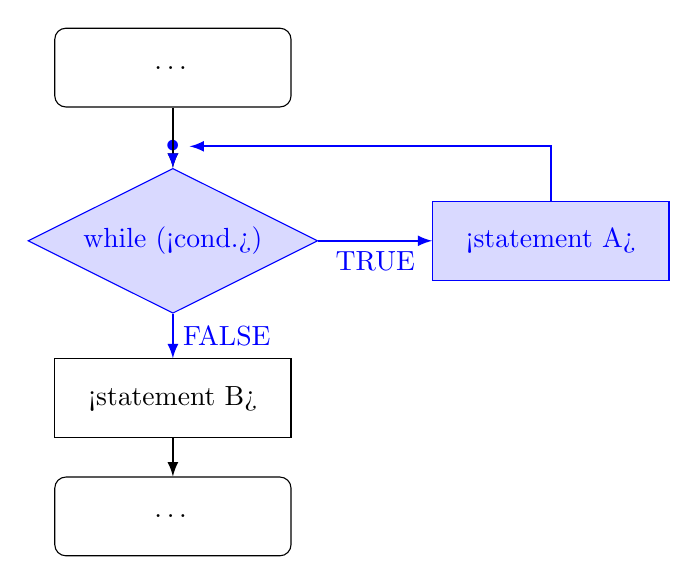
\begin{tikzpicture}[node distance=1.5cm]
\node (start) [startstop] {\ldots};
\node (entry) [below of=start, color = blue, yshift=0.5cm]{$\bullet$};
\node (dec1) [decision, color = blue, fill = blue!15, below of=entry, yshift=0.3cm] {\code{while (<cond.>)}};
\node (stat2) [process, color = blue, fill = blue!15, right of=dec1, xshift=3.3cm] {\code{<statement A>}};
\node (stat3) [process, below of=dec1, yshift=-0.5cm] {\code{<statement B>}};
\node (stop) [startstop, below of=stat3] {\ldots};
\draw [arrow] (start) -- (dec1);
\draw [arrow, color=blue] (dec1) -- node[anchor=north] {\code{TRUE}} (stat2);
\draw [arrow, color=blue] (dec1) -- node[anchor=west] {\code{FALSE}} (stat3);
\draw [arrow, color = blue] (stat2) |- (entry);
\draw [arrow, color = blue] (entry) -- (dec1);
\draw [arrow] (stat3) -- (stop);
\end{tikzpicture}
\end{small}
\end{center}


\begin{knitrout}\footnotesize
\definecolor{shadecolor}{rgb}{0.969, 0.969, 0.969}\color{fgcolor}\begin{kframe}
\begin{alltt}
\hlstd{a} \hlkwb{<-} \hlnum{2}
\hlkwa{while} \hlstd{(a} \hlopt{<} \hlnum{50}\hlstd{) \{}
  \hlkwd{print}\hlstd{(a)}
  \hlstd{a} \hlkwb{<-} \hlstd{a}\hlopt{^}\hlnum{2}
\hlstd{\}}
\end{alltt}
\begin{verbatim}
## [1] 2
## [1] 4
## [1] 16
\end{verbatim}
\begin{alltt}
\hlkwd{print}\hlstd{(a)}
\end{alltt}
\begin{verbatim}
## [1] 256
\end{verbatim}
\end{kframe}
\end{knitrout}

\begin{playground}
Make sure that you understand why the final value of \code{a} is larger than 50.
\end{playground}


\begin{advplayground}
The statements above can be simplified to:

\begin{knitrout}\footnotesize
\definecolor{shadecolor}{rgb}{0.969, 0.969, 0.969}\color{fgcolor}\begin{kframe}
\begin{alltt}
\hlstd{a} \hlkwb{<-} \hlnum{2}
\hlkwd{print}\hlstd{(a)}
\hlkwa{while} \hlstd{(a} \hlopt{<} \hlnum{50}\hlstd{) \{}
  \hlkwd{print}\hlstd{(a} \hlkwb{<-} \hlstd{a}\hlopt{^}\hlnum{2}\hlstd{)}
\hlstd{\}}
\end{alltt}
\end{kframe}
\end{knitrout}

Explain why this works, and how it relates to the support in \Rlang of \emph{chained} assignments to several variables within a single statement like the one below.

\begin{knitrout}\footnotesize
\definecolor{shadecolor}{rgb}{0.969, 0.969, 0.969}\color{fgcolor}\begin{kframe}
\begin{alltt}
\hlstd{a} \hlkwb{<-} \hlstd{b} \hlkwb{<-} \hlstd{c} \hlkwb{<-} \hlnum{1}\hlopt{:}\hlnum{5}
\hlstd{a}
\end{alltt}
\end{kframe}
\end{knitrout}

Explain why a second \code{print(a)} has been added before \code{while()}. Hint: experiment if necessary.
\end{advplayground}

\begin{explainbox}
\Rloop{while} loops as described above will terminate when the condition tested is \code{FALSE}. In those cases that require stopping iteration based on an additional test condition within the compound statement, we can call \Rloop{break()} in the body of an \code{if} or \code{else} statement.
\end{explainbox}

\subsubsection[\texttt{repeat} loops]{\code{repeat} loops}
The \Rloop{repeat}\index{iteration!repeat loop} construct is less frequently used, but adds flexibility as termination will always depend on a call to \Rcontrol{break()}, which can be located anywhere within the compound statement that forms the body of the loop. To achieve conditional end of iteration, function \Rcontrol{break()} must be called, as otherwise, iteration in a \code{repeat} loop will not stop.

\begin{center}
\begin{small}
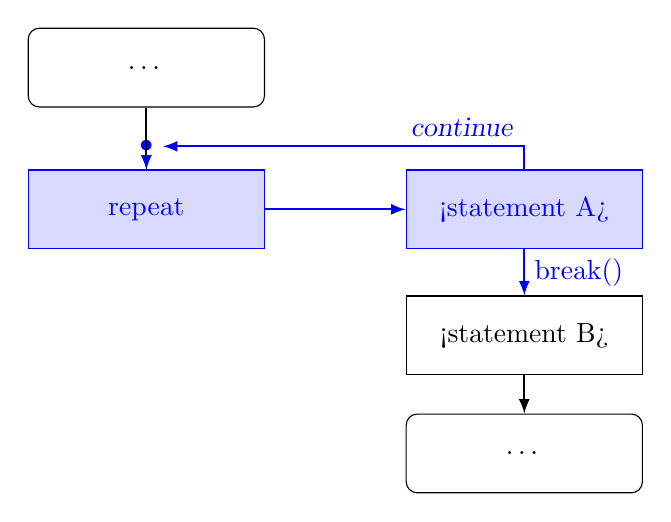
\begin{tikzpicture}[node distance=1.5cm]
\node (start) [startstop] {\ldots};
\node (entry) [below of=start, color = blue, yshift=0.5cm]{$\bullet$};
\node (dec1) [process, color = blue, fill = blue!15, below of=start, yshift=-0.3cm] {\code{repeat}};
\node (stat2) [process, color = blue, fill = blue!15, right of=dec1, xshift=3.3cm] {\code{<statement A>}};
\node (stat3) [process, below of=stat2, yshift=-0.1cm] {\code{<statement B>}};
\node (stop) [startstop, below of=stat3] {\ldots};
\draw [arrow] (start) -- (dec1);
\draw [arrow, color=blue] (dec1) -- node[anchor=north] {} (stat2);
\draw [arrow, color=blue] (stat2) |- node[anchor=south east] {\textsl{continue}} (entry);
\draw [arrow, color=blue] (stat2) -- node[anchor=west] {\code{break()}} (stat3);
\draw [arrow, color = blue] (entry) -- (dec1);
\draw [arrow] (stat3) -- (stop);
\end{tikzpicture}
\end{small}
\end{center}

\begin{knitrout}\footnotesize
\definecolor{shadecolor}{rgb}{0.969, 0.969, 0.969}\color{fgcolor}\begin{kframe}
\begin{alltt}
\hlstd{a} \hlkwb{<-} \hlnum{2}
\hlkwa{repeat}\hlstd{\{}
  \hlkwd{print}\hlstd{(a)}
  \hlkwa{if} \hlstd{(a} \hlopt{>} \hlnum{50}\hlstd{)} \hlkwa{break}\hlstd{()}
  \hlstd{a} \hlkwb{<-} \hlstd{a}\hlopt{^}\hlnum{2}
\hlstd{\}}
\end{alltt}
\begin{verbatim}
## [1] 2
## [1] 4
## [1] 16
## [1] 256
\end{verbatim}
\end{kframe}
\end{knitrout}

\begin{playground}
Please explain why the example above returns the values it does. Use the approach of adding \code{print()} statements, as described on page \pageref{box:play:forloop}.
\end{playground}

\begin{explainbox}
Although \code{repeat} loop constructs are easier to read if they have a single condition resulting in termination of iteration, it is allowed by the \Rlang language for the compound statement in the body of a loop to contain more than one call to \Rcontrol{break()}, each within a different \code{if} or \code{else} statement.

Function \Rcontrol{break()} can be also used within \Rcontrol{for} and \Rcontrol{while} loops. In such case, for clarity, the use of \Rcontrol{break()} should be reserved for exceptional conditions. In a \Rcontrol{for} loop, \Rcontrol{next()} interrupts the current iteration and jumps to the start of the next one.
\end{explainbox}

\subsection{Explicit loops can be slow in \Rlang}\label{sec:loops:slow}
\index{vectorization}\index{recycling of arguments}\index{iteration}\index{loops!faster alternatives|(}
If you have written programs in other languages, it will feel natural to you to use loops (\Rloop{for}, \Rloop{while}, \Rloop{repeat}) for many of the things for which in \Rlang one would normally use vectorization. In \Rlang, using vectorization whenever possible keeps scripts shorter and easier to understand (at least for those with experience in \Rlang). More importantly, as \Rlang is an interpreted language, vectorized arithmetic tends to be much faster than the use of explicit iteration. In recent versions of \Rpgrm, byte-compilation is used by default and loops may be compiled on the fly, which relieves part of the burden of repeated interpretation. However, even byte-compiled loops are usually slower to execute than efficiently coded vectorized functions and operators.

Execution speed needs to be balanced against the effort invested in writing faster code. However, using vectorization and specific \Rlang functions requires little effort once we are familiar with them. The simplest way of measuring the execution time of an \Rlang expression is to use function \Rfunction{system.time()}. However, the returned time is in seconds and consequently the expression must take long enough to execute for the returned time to have useful resolution. See package \pkgname{microbenchmark} for tools for benchmarking code with better time resolution.\qRloop{for}

\begin{knitrout}\footnotesize
\definecolor{shadecolor}{rgb}{0.969, 0.969, 0.969}\color{fgcolor}\begin{kframe}
\begin{alltt}
\hlkwd{system.time}\hlstd{(\{a} \hlkwb{<-} \hlkwd{numeric}\hlstd{()}
            \hlkwa{for} \hlstd{(i} \hlkwa{in} \hlnum{1}\hlopt{:}\hlnum{1000000}\hlstd{) \{}
              \hlstd{a[i]} \hlkwb{<-} \hlstd{i} \hlopt{/} \hlnum{1000}
              \hlstd{\}}
            \hlstd{\})}
\end{alltt}
\begin{verbatim}
##    user  system elapsed 
##    0.25    0.01    0.27
\end{verbatim}
\end{kframe}
\end{knitrout}

\begin{explainbox}
Whenever\label{box:vectorization:perf} working with large data sets, or many similar data sets, we will need to take performance into account. As vectorization usually also makes code simpler, it is good style to use vectorization whenever possible. For operations that are frequently used, \Rlang includes specific functions. It is thus important to consider not only vectorization of arithmetic but also check for the availability of performance-optimized functions for specific cases. The results from running the code examples in this box are not included, because they are the same for all chunks. Here we are interested in the execution time, and we leave this as an exercise.

\begin{knitrout}\footnotesize
\definecolor{shadecolor}{rgb}{0.969, 0.969, 0.969}\color{fgcolor}\begin{kframe}
\begin{alltt}
\hlstd{a} \hlkwb{<-} \hlkwd{rnorm}\hlstd{(}\hlnum{10}\hlopt{^}\hlnum{7}\hlstd{)} \hlcom{# 10 000 0000 pseudo-random numbers}
\end{alltt}
\end{kframe}
\end{knitrout}

\begin{knitrout}\footnotesize
\definecolor{shadecolor}{rgb}{0.969, 0.969, 0.969}\color{fgcolor}\begin{kframe}
\begin{alltt}
\hlcom{# b <- numeric()}
\hlstd{b} \hlkwb{<-} \hlkwd{numeric}\hlstd{(}\hlkwd{length}\hlstd{(a)}\hlopt{-}\hlnum{1}\hlstd{)} \hlcom{# pre-allocate memory}
\hlstd{i} \hlkwb{<-} \hlnum{1}
\hlkwa{while} \hlstd{(i} \hlopt{<} \hlkwd{length}\hlstd{(a)) \{}
  \hlstd{b[i]} \hlkwb{<-} \hlstd{a[i}\hlopt{+}\hlnum{1}\hlstd{]} \hlopt{-} \hlstd{a[i]}
  \hlkwd{print}\hlstd{(b)}
  \hlstd{i} \hlkwb{<-} \hlstd{i} \hlopt{+} \hlnum{1}
\hlstd{\}}
\hlstd{b}
\end{alltt}
\end{kframe}
\end{knitrout}

\begin{knitrout}\footnotesize
\definecolor{shadecolor}{rgb}{0.969, 0.969, 0.969}\color{fgcolor}\begin{kframe}
\begin{alltt}
\hlcom{# b <- numeric()}
\hlstd{b} \hlkwb{<-} \hlkwd{numeric}\hlstd{(}\hlkwd{length}\hlstd{(a)}\hlopt{-}\hlnum{1}\hlstd{)} \hlcom{# pre-allocate memory}
\hlkwa{for}\hlstd{(i} \hlkwa{in} \hlkwd{seq}\hlstd{(}\hlkwc{along.with} \hlstd{= b)) \{}
  \hlstd{b[i]} \hlkwb{<-} \hlstd{a[i}\hlopt{+}\hlnum{1}\hlstd{]} \hlopt{-} \hlstd{a[i]}
  \hlkwd{print}\hlstd{(b)}
\hlstd{\}}
\hlstd{b}
\end{alltt}
\end{kframe}
\end{knitrout}

\begin{knitrout}\footnotesize
\definecolor{shadecolor}{rgb}{0.969, 0.969, 0.969}\color{fgcolor}\begin{kframe}
\begin{alltt}
\hlcom{# although in this case there were alternatives, there}
\hlcom{# are other cases when we need to use indexes explicitly}
\hlstd{b} \hlkwb{<-} \hlstd{a[}\hlnum{2}\hlopt{:}\hlkwd{length}\hlstd{(a)]} \hlopt{-} \hlstd{a[}\hlnum{1}\hlopt{:}\hlkwd{length}\hlstd{(a)}\hlopt{-}\hlnum{1}\hlstd{]}
\hlstd{b}
\end{alltt}
\end{kframe}
\end{knitrout}

\begin{knitrout}\footnotesize
\definecolor{shadecolor}{rgb}{0.969, 0.969, 0.969}\color{fgcolor}\begin{kframe}
\begin{alltt}
\hlcom{# or even better}
\hlstd{b} \hlkwb{<-} \hlkwd{diff}\hlstd{(a)}
\hlstd{b}
\end{alltt}
\end{kframe}
\end{knitrout}

Execution time can be obtained with \Rfunction{system.time()}. For a vector of ten million numbers, the \code{for} loop above takes 1.1\,s and the equivalent \code{while} loop 2.0\,s, the vectorized statement using indexing takes 0.2\,s and function \code{diff()} takes 0.1\,s. The \code{for} loop without pre-allocation of memory to \code{b} takes 3.6\,s, and the equivalent while loop 4.7\,s---i.e., the fastest execution time was more than 40 times faster than the slowest one. (Times for \Rpgrm 3.5.1 on my laptop under Windows 10 x64.)
\end{explainbox}
\index{loops!faster alternatives|)}

\subsection{Nesting of loops}\label{sec:nested:loops}
\index{iteration!nesting of loops}\index{nested iteration loops}\index{loops!nested}

All the execution-flow control statements seen above can be nested. We will show an example with two \code{for} loops. We first create a matrix of data to work with:

\begin{knitrout}\footnotesize
\definecolor{shadecolor}{rgb}{0.969, 0.969, 0.969}\color{fgcolor}\begin{kframe}
\begin{alltt}
\hlstd{A} \hlkwb{<-} \hlkwd{matrix}\hlstd{(}\hlnum{1}\hlopt{:}\hlnum{50}\hlstd{,} \hlnum{10}\hlstd{)}
\hlstd{A}
\end{alltt}
\begin{verbatim}
##       [,1] [,2] [,3] [,4] [,5]
##  [1,]    1   11   21   31   41
##  [2,]    2   12   22   32   42
##  [3,]    3   13   23   33   43
##  [4,]    4   14   24   34   44
##  [5,]    5   15   25   35   45
##  [6,]    6   16   26   36   46
##  [7,]    7   17   27   37   47
##  [8,]    8   18   28   38   48
##  [9,]    9   19   29   39   49
## [10,]   10   20   30   40   50
\end{verbatim}
\end{kframe}
\end{knitrout}

\begin{knitrout}\footnotesize
\definecolor{shadecolor}{rgb}{0.969, 0.969, 0.969}\color{fgcolor}\begin{kframe}
\begin{alltt}
\hlstd{row.sum} \hlkwb{<-} \hlkwd{numeric}\hlstd{()}
\hlkwa{for} \hlstd{(i} \hlkwa{in} \hlnum{1}\hlopt{:}\hlkwd{nrow}\hlstd{(A)) \{}
  \hlstd{row.sum[i]} \hlkwb{<-} \hlnum{0}
  \hlkwa{for} \hlstd{(j} \hlkwa{in} \hlnum{1}\hlopt{:}\hlkwd{ncol}\hlstd{(A))}
    \hlstd{row.sum[i]} \hlkwb{<-} \hlstd{row.sum[i]} \hlopt{+} \hlstd{A[i, j]}
\hlstd{\}}
\hlkwd{print}\hlstd{(row.sum)}
\end{alltt}
\begin{verbatim}
##  [1] 105 110 115 120 125 130 135 140 145 150
\end{verbatim}
\end{kframe}
\end{knitrout}

The code above is very general, it will work with any two-dimensional matrix with at least one column and one row. However, sometimes we need more specific calculations. \code{A[1, 2]} selects one cell in the matrix, the one on the first row of the second column. \code{A[1, ]} selects row one, and  \code{A[ , 2]} selects column two. In the example above, the value of \code{i} changes for each iteration of the outer loop. The value of \code{j} changes for each iteration of the inner loop, and the inner loop is run in full for each iteration of the outer loop. The inner loop index \code{j} changes fastest.

\begin{advplayground}
1) Modify the code in the example in the last chunk above so that it sums the values only in the first three columns of \code{A}, 2) modify the same example so that it sums the values only in the last three rows of \code{A}, 3) modify the code so that matrices with dimensions equal to zero (as reported by \code{ncol()} and \code{nrow()}).

Will the code you wrote continue working as expected if the number of rows in \code{A} changed? What if the number of columns in \code{A} changed, and the required results still needed to be calculated for relative positions? What would happen if \code{A} had fewer than three columns? Try to think first what to expect based on the code you wrote. Then create matrices of different sizes and test your code. After that, think how to improve the code, so that wrong results are not produced.
\end{advplayground}

\begin{explainbox}
If the total number of iterations is large and the code executed at each iteration runs fast, the overhead added by the loop code can make a big contribution to the total running time of a script.
When dealing with nested loops, as the inner loop is executed most frequently, this is the best place to look for ways of reducing execution time. In this example, vectorization can be achieved easily for the inner loop, as \Rlang has a function \code{sum()} which returns the sum of a vector passed as its argument. Replacing the inner loop by an efficient function can be expected to improve performance significantly.

\begin{knitrout}\footnotesize
\definecolor{shadecolor}{rgb}{0.969, 0.969, 0.969}\color{fgcolor}\begin{kframe}
\begin{alltt}
\hlstd{row.sum} \hlkwb{<-} \hlkwd{numeric}\hlstd{(}\hlkwd{nrow}\hlstd{(A))} \hlcom{# faster}
\hlkwa{for} \hlstd{(i} \hlkwa{in} \hlnum{1}\hlopt{:}\hlkwd{nrow}\hlstd{(A)) \{}
  \hlstd{row.sum[i]} \hlkwb{<-} \hlkwd{sum}\hlstd{(A[i, ])}
\hlstd{\}}
\hlkwd{print}\hlstd{(row.sum)}
\end{alltt}
\begin{verbatim}
##  [1] 105 110 115 120 125 130 135 140 145 150
\end{verbatim}
\end{kframe}
\end{knitrout}

\code{A[i, ]} selects row \code{i} and all columns. Reminder: in \Rlang the row index comes first.

Both\index{apply functions} explicit loops can be eliminated if we use an \emph{apply} function, such as \Rloop{apply()}, \Rloop{lapply()} or \Rloop{sapply()}, in place of the outer \code{for} loop. See section \ref{sec:data:apply} below %on page \pageref{sec:data:apply}
for details on the use of the different \emph{apply} functions.

\begin{knitrout}\footnotesize
\definecolor{shadecolor}{rgb}{0.969, 0.969, 0.969}\color{fgcolor}\begin{kframe}
\begin{alltt}
\hlstd{row.sum} \hlkwb{<-} \hlkwd{apply}\hlstd{(A,} \hlkwc{MARGIN} \hlstd{=} \hlnum{1}\hlstd{, sum)} \hlcom{# MARGIN=1 indicates rows}
\hlkwd{print}\hlstd{(row.sum)}
\end{alltt}
\begin{verbatim}
##  [1] 105 110 115 120 125 130 135 140 145 150
\end{verbatim}
\end{kframe}
\end{knitrout}
Calculating row sums is a frequent operation, so \Rlang has a built-in function for this. As earlier with \code{diff()}, it is always worthwhile to check if there is an existing \Rlang function, optimized for performance, capable of doing the computations we need. In this case, using \code{rowSums()} simplifies the nested loops into a single function call, both improving performance and readability.

\begin{knitrout}\footnotesize
\definecolor{shadecolor}{rgb}{0.969, 0.969, 0.969}\color{fgcolor}\begin{kframe}
\begin{alltt}
\hlkwd{rowSums}\hlstd{(A)}
\end{alltt}
\begin{verbatim}
##  [1] 105 110 115 120 125 130 135 140 145 150
\end{verbatim}
\end{kframe}
\end{knitrout}

\end{explainbox}

\begin{playground}
1) How would you change this last example, so that only the last three columns are added up? (Think about use of subscripts to select a part of the matrix.)
2) To obtain column sums, one could modify the nested loops (think how), transpose the matrix and use \code{rowSums()} (think how), or look up if there is in \Rlang a function for this operation. A good place to start is with \code{help(rowSums)} as similar functions may share the same help page, or at least be listed in the ``See also'' section. Do try this, and explore other help pages in search for some function you may find useful in the analysis of your own data.
\end{playground}

\subsubsection{Clean-up}

Sometimes we need to make sure that clean-up code is executed even if the execution of a script or function is aborted by the user or as a result of an error condition. A typical example is a script that temporarily sets a disk folder as the working directory or uses a file as temporary storage. Function \Rfunction{on.exit()} can be used to record that a user supplied expression needs to be executed when the current function, or a script, exits. Function \Rfunction{on.exit()} can also make code easier to read as it keeps creation and clean-up next to each other in the body of a function or in the listing of a script.

\begin{knitrout}\footnotesize
\definecolor{shadecolor}{rgb}{0.969, 0.969, 0.969}\color{fgcolor}\begin{kframe}
\begin{alltt}
\hlkwd{file.create}\hlstd{(}\hlstr{"temp.file"}\hlstd{)}
\end{alltt}
\begin{verbatim}
## [1] TRUE
\end{verbatim}
\begin{alltt}
\hlkwd{on.exit}\hlstd{(}\hlkwd{file.remove}\hlstd{(}\hlstr{"temp.file"}\hlstd{))}
\hlcom{# code that makes use of the file goes here}
\end{alltt}
\end{kframe}
\end{knitrout}

\section[Apply functions]{\emph{Apply} functions}\label{sec:data:apply}

\emph{Apply}\index{apply functions}\index{loops!faster alternatives} functions apply a function passed as an argument to parameter \code{FUN} or equivalent, to elements in a collection of \Rlang objects passed as an argument to parameter \code{X} or equivalent. Collections to which \code{FUN} is to be applied can be vectors, lists, data frames, matrices or arrays. As long as the operations to be applied are \emph{independent---i.e., the results from one iteration are not used in another iteration---} apply functions can replace \code{for}, \code{while} or \code{repeat} loops.

\begin{explainbox}
Conceptually, \code{for}, \code{while} and \code{repeat} loops are interpreted as controlling sequential evaluation of program statements. In contrast, \Rlang's \emph{apply} functions are, conceptually, thought as evaluating a function in parallel for each of the different members of their input. So, while in loops the results of earlier iterations through a loop can be stored in variables and used in subsequent iterations, this is not possible in the case of \emph{apply} functions.
\end{explainbox}

The different \emph{apply} functions in base \Rlang differ in the class of the values they accept for their \code{X} parameter, the class of the object they return and/or the class of the value returned by the applied function. \Rloop{lapply()} and \Rloop{sapply()} expect a \code{vector} or \code{list} as an argument passed through \code{X}. \Rloop{lapply()} returns a \code{list} or an \code{array}; and \Rloop{vapply()} always \emph{simplifies} its returned value into a vector, while \Rloop{sapply()} does the simplification according to the argument passed to its \code{simplify} parameter. All these \emph{apply} functions can be used to apply an \Rlang function that returns a value of the same or a different class as its argument. In the case of \Rloop{apply()} and \Rloop{lapply()} not even the length of the values returned for each member of the collection passed as an argument, needs to be consistent. In summary, \Rloop{apply()} is used to apply a function to the elements along a dimension of an object that has two or more \emph{dimensions}, and \Rloop{lapply()} and \Rloop{sapply()} are used to apply a function to the members of a vector or list. \Rloop{apply()} returns an array or a list or a vector depending on the size, and consistency in length and class among the values returned by the applied function.

\subsection{Applying functions to vectors and lists}

We first exemplify the use of \Rloop{lapply()}, \Rloop{sapply()} and \Rloop{vapply()}. In the chunks below we apply a user-defined function to a vector.

\begin{warningbox}
A constraint is that the individual member objects in the list or vector passed as argument to the \code{x} parameter of \textit{apply} functions will be always passed as a positional argument to the first formal parameter of the applied function, i.e., the function passed as argument to \code{FUN} must be compatible with this approach.
\end{warningbox}

\begin{knitrout}\footnotesize
\definecolor{shadecolor}{rgb}{0.969, 0.969, 0.969}\color{fgcolor}\begin{kframe}
\begin{alltt}
\hlkwd{set.seed}\hlstd{(}\hlnum{123456}\hlstd{)} \hlcom{# so that a.vector does not change}
\hlstd{a.vector} \hlkwb{<-} \hlkwd{runif}\hlstd{(}\hlnum{6}\hlstd{)} \hlcom{# A short vector as input to keep output short}
\hlkwd{str}\hlstd{(a.vector)}
\end{alltt}
\begin{verbatim}
##  num [1:6] 0.798 0.754 0.391 0.342 0.361 ...
\end{verbatim}
\end{kframe}
\end{knitrout}

\begin{knitrout}\footnotesize
\definecolor{shadecolor}{rgb}{0.969, 0.969, 0.969}\color{fgcolor}\begin{kframe}
\begin{alltt}
\hlstd{my.fun} \hlkwb{<-} \hlkwa{function}\hlstd{(}\hlkwc{x}\hlstd{,} \hlkwc{k}\hlstd{) \{}\hlkwd{log}\hlstd{(x)} \hlopt{+} \hlstd{k\}}
\end{alltt}
\end{kframe}
\end{knitrout}

\begin{knitrout}\footnotesize
\definecolor{shadecolor}{rgb}{0.969, 0.969, 0.969}\color{fgcolor}\begin{kframe}
\begin{alltt}
\hlstd{z} \hlkwb{<-} \hlkwd{lapply}\hlstd{(}\hlkwc{X} \hlstd{= a.vector,} \hlkwc{FUN} \hlstd{= my.fun,} \hlkwc{k} \hlstd{=} \hlnum{5}\hlstd{)}
\hlkwd{str}\hlstd{(z)}
\end{alltt}
\begin{verbatim}
## List of 6
##  $ : num 4.77
##  $ : num 4.72
##  $ : num 4.06
##  $ : num 3.93
##  $ : num 3.98
##  $ : num 3.38
\end{verbatim}
\end{kframe}
\end{knitrout}

\begin{knitrout}\footnotesize
\definecolor{shadecolor}{rgb}{0.969, 0.969, 0.969}\color{fgcolor}\begin{kframe}
\begin{alltt}
\hlstd{z} \hlkwb{<-} \hlkwd{sapply}\hlstd{(}\hlkwc{X} \hlstd{= a.vector,} \hlkwc{FUN} \hlstd{= my.fun,} \hlkwc{k} \hlstd{=} \hlnum{5}\hlstd{)}
\hlkwd{str}\hlstd{(z)}
\end{alltt}
\begin{verbatim}
##  num [1:6] 4.77 4.72 4.06 3.93 3.98 ...
\end{verbatim}
\end{kframe}
\end{knitrout}

\begin{knitrout}\footnotesize
\definecolor{shadecolor}{rgb}{0.969, 0.969, 0.969}\color{fgcolor}\begin{kframe}
\begin{alltt}
\hlstd{z} \hlkwb{<-} \hlkwd{sapply}\hlstd{(}\hlkwc{X} \hlstd{= a.vector,} \hlkwc{FUN} \hlstd{= my.fun,} \hlkwc{k} \hlstd{=} \hlnum{5}\hlstd{,} \hlkwc{simplify} \hlstd{=} \hlnum{FALSE}\hlstd{)}
\hlkwd{str}\hlstd{(z)}
\end{alltt}
\begin{verbatim}
## List of 6
##  $ : num 4.77
##  $ : num 4.72
##  $ : num 4.06
##  $ : num 3.93
##  $ : num 3.98
##  $ : num 3.38
\end{verbatim}
\end{kframe}
\end{knitrout}

We can see above that the computed results are the same in the three cases, but the class and structure of the objects returned differ.

Anonymous functions can be defined on the fly and passed to \code{FUN}, allowing us to re-write the examples above more concisely (only the second one shown).

\begin{knitrout}\footnotesize
\definecolor{shadecolor}{rgb}{0.969, 0.969, 0.969}\color{fgcolor}\begin{kframe}
\begin{alltt}
\hlstd{z} \hlkwb{<-} \hlkwd{sapply}\hlstd{(}\hlkwc{X} \hlstd{= a.vector,} \hlkwc{FUN} \hlstd{=} \hlkwa{function}\hlstd{(}\hlkwc{x}\hlstd{,} \hlkwc{k}\hlstd{) \{}\hlkwd{log}\hlstd{(x)} \hlopt{+} \hlstd{k\},} \hlkwc{k} \hlstd{=} \hlnum{5}\hlstd{)}
\hlkwd{str}\hlstd{(z)}
\end{alltt}
\begin{verbatim}
##  num [1:6] 4.77 4.72 4.06 3.93 3.98 ...
\end{verbatim}
\end{kframe}
\end{knitrout}

Of course, as discussed in section \ref{sec:loops:slow} on page \pageref{sec:loops:slow}, when suitable vectorized functions are available, their use should be preferred. On the other hand, even if \emph{apply} functions are usually not as fast as vectorized functions, they are faster than the equivalent \code{for()} loops.

\begin{knitrout}\footnotesize
\definecolor{shadecolor}{rgb}{0.969, 0.969, 0.969}\color{fgcolor}\begin{kframe}
\begin{alltt}
\hlstd{z} \hlkwb{<-} \hlkwd{log}\hlstd{(a.vector)} \hlopt{+} \hlnum{5}
\hlkwd{str}\hlstd{(z)}
\end{alltt}
\begin{verbatim}
##  num [1:6] 4.77 4.72 4.06 3.93 3.98 ...
\end{verbatim}
\end{kframe}
\end{knitrout}

\begin{explainbox}
Function \Rloop{vapply()} can be safer to use as the mode of returned values is enforced. Here is a possible way of obtaining means and variances across member vectors at each vector index position from a list of vectors. These could be called \emph{parallel} means and variances. The argument passed to \code{FUN.VALUE} provides a template for the type of the return value and its organization into rows and columns. Notice that the rows in the output are now named according to the names in \code{FUN.VALUE}.

We first use \code{lapply()} to create the object \code{a.list} containing artificial data. One or more additional \emph{named} arguments can be passed to the function to be applied.

\begin{knitrout}\footnotesize
\definecolor{shadecolor}{rgb}{0.969, 0.969, 0.969}\color{fgcolor}\begin{kframe}
\begin{alltt}
\hlkwd{set.seed}\hlstd{(}\hlnum{123456}\hlstd{)}
\hlstd{a.list} \hlkwb{<-} \hlkwd{lapply}\hlstd{(}\hlkwd{rep}\hlstd{(}\hlnum{4}\hlstd{,} \hlnum{5}\hlstd{), rnorm,} \hlkwc{mean} \hlstd{=} \hlnum{10}\hlstd{,} \hlkwc{sd} \hlstd{=} \hlnum{1}\hlstd{)}
\hlkwd{str}\hlstd{(a.list)}
\end{alltt}
\begin{verbatim}
## List of 5
##  $ : num [1:4] 10.83 9.72 9.64 10.09
##  $ : num [1:4] 12.3 10.8 11.3 12.5
##  $ : num [1:4] 11.17 9.57 9 8.89
##  $ : num [1:4] 9.94 11.17 11.05 10.06
##  $ : num [1:4] 9.26 10.93 11.67 10.56
\end{verbatim}
\end{kframe}
\end{knitrout}

We define the function that we will apply, a function that returns a numeric vector of length 2.

\begin{knitrout}\footnotesize
\definecolor{shadecolor}{rgb}{0.969, 0.969, 0.969}\color{fgcolor}\begin{kframe}
\begin{alltt}
\hlstd{mean_and_sd} \hlkwb{<-} \hlkwa{function}\hlstd{(}\hlkwc{x}\hlstd{,} \hlkwc{na.rm} \hlstd{=} \hlnum{FALSE}\hlstd{) \{}
       \hlkwd{c}\hlstd{(}\hlkwd{mean}\hlstd{(x,} \hlkwc{na.rm} \hlstd{= na.rm),}  \hlkwd{sd}\hlstd{(x,} \hlkwc{na.rm} \hlstd{= na.rm))}
    \hlstd{\}}
\end{alltt}
\end{kframe}
\end{knitrout}

We next use \Rloop{vapply()} to apply our function to each member vector of the list.

\begin{knitrout}\footnotesize
\definecolor{shadecolor}{rgb}{0.969, 0.969, 0.969}\color{fgcolor}\begin{kframe}
\begin{alltt}
\hlstd{values} \hlkwb{<-} \hlkwd{vapply}\hlstd{(}\hlkwc{X} \hlstd{= a.list,}
                 \hlkwc{FUN} \hlstd{= mean_and_sd,}
                 \hlkwc{FUN.VALUE} \hlstd{=} \hlkwd{c}\hlstd{(}\hlkwc{mean} \hlstd{=} \hlnum{0}\hlstd{,} \hlkwc{sd} \hlstd{=} \hlnum{0}\hlstd{),}
                 \hlkwc{na.rm} \hlstd{=} \hlnum{TRUE}\hlstd{)}
\hlkwd{class}\hlstd{(values)}
\end{alltt}
\begin{verbatim}
## [1] "matrix" "array"
\end{verbatim}
\begin{alltt}
\hlstd{values}
\end{alltt}
\begin{verbatim}
##            [,1]       [,2]     [,3]       [,4]      [,5]
## mean 10.0725427 11.7254442 9.657997 10.5573814 10.605846
## sd    0.5428149  0.7844356 1.050663  0.6460881  1.005676
\end{verbatim}
\end{kframe}
\end{knitrout}
\end{explainbox}

\begin{playground}
As explained in section \ref{sec:R:data:frames} on page \pageref{sec:R:data:frames}, class \code{data.frame} is derived from class \code{list}. Apply function \code{mean\_and\_sd()} defined above to the data frame \code{cars} included as example data in \Rlang. The aim is to obtain the mean and standard deviation for each column.
\end{playground}

\subsection{Applying functions to matrices and arrays}
In the next example we use \Rloop{apply()} and \Rfunction{mean()} to compute the mean for each column of matrix \code{a.matrix}. In \Rlang the dimensions of a matrix, rows and columns, over which a function is applied are called \emph{margins}. The argument passed to parameter \code{MARGIN} determines over which margin the function will be applied. If the function is applied to individual rows, we say that we operate on the first margin, and if the function is applied to individual columns, over the second margin. Arrays can have many dimensions, and consequently more margins. In the case of arrays with more than two dimensions, it is possible and useful to apply functions over multiple margins at once.

\begin{warningbox}
A constraint on the function to be applied is that the vector or ``slice'' will always be passed as a positional argument to the first formal parameter of the applied function.
\end{warningbox}

\begin{knitrout}\footnotesize
\definecolor{shadecolor}{rgb}{0.969, 0.969, 0.969}\color{fgcolor}\begin{kframe}
\begin{alltt}
\hlstd{a.matrix} \hlkwb{<-} \hlkwd{matrix}\hlstd{(}\hlkwd{runif}\hlstd{(}\hlnum{100}\hlstd{),} \hlkwc{ncol} \hlstd{=} \hlnum{10}\hlstd{)}
\hlstd{z} \hlkwb{<-} \hlkwd{apply}\hlstd{(a.matrix,} \hlkwc{MARGIN} \hlstd{=} \hlnum{1}\hlstd{,} \hlkwc{FUN} \hlstd{= mean)}
\hlkwd{str}\hlstd{(z)}
\end{alltt}
\begin{verbatim}
##  num [1:10] 0.247 0.404 0.537 0.5 0.504 ...
\end{verbatim}
\end{kframe}
\end{knitrout}

\begin{playground}
Modify the example above so that it computes row means instead of column means.
\end{playground}

\begin{playground}
Look up the help pages for \Rloop{apply()} and \code{mean()} and study them until you understand how additional arguments can be passed to the applied function. Can you guess why \Rloop{apply()} was designed to have parameter names fully in uppercase, something very unusual for \Rlang code style?
\end{playground}

If we apply a function that returns a value of the same length as its input, then the dimensions of the value returned by \Rloop{apply()} are the same as those of its input. We use, in the next examples, a ``no-op'' function that returns its argument unchanged, so that input and output can be easily compared.

\begin{knitrout}\footnotesize
\definecolor{shadecolor}{rgb}{0.969, 0.969, 0.969}\color{fgcolor}\begin{kframe}
\begin{alltt}
\hlstd{a.small.matrix} \hlkwb{<-} \hlkwd{matrix}\hlstd{(}\hlkwd{rnorm}\hlstd{(}\hlnum{6}\hlstd{,} \hlkwc{mean} \hlstd{=} \hlnum{10}\hlstd{,} \hlkwc{sd} \hlstd{=} \hlnum{1}\hlstd{),} \hlkwc{ncol} \hlstd{=} \hlnum{2}\hlstd{)}
\hlstd{a.small.matrix} \hlkwb{<-} \hlkwd{round}\hlstd{(a.small.matrix,} \hlkwc{digits} \hlstd{=} \hlnum{1}\hlstd{)}
\hlstd{a.small.matrix}
\end{alltt}
\begin{verbatim}
##      [,1] [,2]
## [1,] 11.3 10.4
## [2,] 10.6  8.6
## [3,]  8.2 11.0
\end{verbatim}
\end{kframe}
\end{knitrout}

\begin{knitrout}\footnotesize
\definecolor{shadecolor}{rgb}{0.969, 0.969, 0.969}\color{fgcolor}\begin{kframe}
\begin{alltt}
\hlstd{no_op.fun} \hlkwb{<-} \hlkwa{function}\hlstd{(}\hlkwc{x}\hlstd{) \{x\}}
\end{alltt}
\end{kframe}
\end{knitrout}

\begin{knitrout}\footnotesize
\definecolor{shadecolor}{rgb}{0.969, 0.969, 0.969}\color{fgcolor}\begin{kframe}
\begin{alltt}
\hlstd{z} \hlkwb{<-} \hlkwd{apply}\hlstd{(}\hlkwc{X} \hlstd{= a.small.matrix,} \hlkwc{MARGIN} \hlstd{=} \hlnum{2}\hlstd{,} \hlkwc{FUN} \hlstd{= no_op.fun)}
\hlkwd{class}\hlstd{(z)}
\end{alltt}
\begin{verbatim}
## [1] "matrix" "array"
\end{verbatim}
\begin{alltt}
\hlstd{z}
\end{alltt}
\begin{verbatim}
##      [,1] [,2]
## [1,] 11.3 10.4
## [2,] 10.6  8.6
## [3,]  8.2 11.0
\end{verbatim}
\end{kframe}
\end{knitrout}

In the chunk above, we passed \code{MARGIN = 2}, but if we pass \code{MARGIN = 1}, we get a return value that is transposed! To restore the original layout of the matrix we can transpose the result with function \Rfunction{t()}.

\begin{knitrout}\footnotesize
\definecolor{shadecolor}{rgb}{0.969, 0.969, 0.969}\color{fgcolor}\begin{kframe}
\begin{alltt}
\hlstd{z} \hlkwb{<-} \hlkwd{apply}\hlstd{(}\hlkwc{X} \hlstd{= a.small.matrix,} \hlkwc{MARGIN} \hlstd{=} \hlnum{1}\hlstd{,} \hlkwc{FUN} \hlstd{= no_op.fun)}
\hlstd{z}
\end{alltt}
\begin{verbatim}
##      [,1] [,2] [,3]
## [1,] 11.3 10.6  8.2
## [2,] 10.4  8.6 11.0
\end{verbatim}
\begin{alltt}
\hlkwd{t}\hlstd{(z)}
\end{alltt}
\begin{verbatim}
##      [,1] [,2]
## [1,] 11.3 10.4
## [2,] 10.6  8.6
## [3,]  8.2 11.0
\end{verbatim}
\end{kframe}
\end{knitrout}

A more realistic example, but difficult to grasp without seeing the toy examples shown above, is when we apply a function that returns a value of a different length than its input, but longer than one. When we compute column summaries (\code{MARGIN = 2}), a matrix is returned, with each column containing the summaries for the corresponding column in the original matrix (\code{a.small.matrix}). In contrast, when we compute row summaries (\code{MARGIN = 1}), each column in the returned matrix contains the summaries for one row in the original array. What happens is that by using \Rloop{apply()} the dimension of the original matrix or array over which we compute summaries ``disappears.'' Consequently, given how matrices are stored in \Rlang, when columns collapse into a single value, the rows become columns. After this, the vectors returned by the applied function, are stored as rows.

\begin{knitrout}\footnotesize
\definecolor{shadecolor}{rgb}{0.969, 0.969, 0.969}\color{fgcolor}\begin{kframe}
\begin{alltt}
\hlstd{mean_and_sd} \hlkwb{<-} \hlkwa{function}\hlstd{(}\hlkwc{x}\hlstd{,} \hlkwc{na.rm} \hlstd{=} \hlnum{FALSE}\hlstd{) \{}
       \hlkwd{c}\hlstd{(}\hlkwd{mean}\hlstd{(x,} \hlkwc{na.rm} \hlstd{= na.rm),}  \hlkwd{sd}\hlstd{(x,} \hlkwc{na.rm} \hlstd{= na.rm))}
    \hlstd{\}}
\end{alltt}
\end{kframe}
\end{knitrout}

\begin{knitrout}\footnotesize
\definecolor{shadecolor}{rgb}{0.969, 0.969, 0.969}\color{fgcolor}\begin{kframe}
\begin{alltt}
\hlstd{z} \hlkwb{<-} \hlkwd{apply}\hlstd{(}\hlkwc{X} \hlstd{= a.small.matrix,} \hlkwc{MARGIN} \hlstd{=} \hlnum{2}\hlstd{,} \hlkwc{FUN} \hlstd{= mean_and_sd,} \hlkwc{na.rm} \hlstd{=} \hlnum{TRUE}\hlstd{)}
\hlstd{z}
\end{alltt}
\begin{verbatim}
##           [,1]   [,2]
## [1,] 10.033333 10.000
## [2,]  1.625833  1.249
\end{verbatim}
\end{kframe}
\end{knitrout}

\begin{knitrout}\footnotesize
\definecolor{shadecolor}{rgb}{0.969, 0.969, 0.969}\color{fgcolor}\begin{kframe}
\begin{alltt}
\hlstd{z} \hlkwb{<-} \hlkwd{apply}\hlstd{(}\hlkwc{X} \hlstd{= a.small.matrix,} \hlkwc{MARGIN} \hlstd{=} \hlnum{1}\hlstd{,} \hlkwc{FUN} \hlstd{= mean_and_sd,} \hlkwc{na.rm} \hlstd{=} \hlnum{TRUE}\hlstd{)}
\hlstd{z}
\end{alltt}
\begin{verbatim}
##            [,1]     [,2]     [,3]
## [1,] 10.8500000 9.600000 9.600000
## [2,]  0.6363961 1.414214 1.979899
\end{verbatim}
\end{kframe}
\end{knitrout}

In all examples above, we have used ordinary functions. Operators in \Rlang are functions with two formal parameters which can be called using infix notation in expressions---i.e., \code{a + b}. By back-quoting their names they can be called using the same syntax as for ordinary functions, and consequently also passed to the \code{FUN} parameter of apply functions. A toy example, equivalent to the vectorized operation \code{a.vector + 5} follows. We enclosed operator \code{+} in back ticks (\code{`}) and pass by name a constant to its second formal parameter (\code{e2 = 5}).

\begin{knitrout}\footnotesize
\definecolor{shadecolor}{rgb}{0.969, 0.969, 0.969}\color{fgcolor}\begin{kframe}
\begin{alltt}
\hlkwd{set.seed}\hlstd{(}\hlnum{123456}\hlstd{)} \hlcom{# so that a.vector does not change}
\hlstd{a.vector} \hlkwb{<-} \hlkwd{runif}\hlstd{(}\hlnum{10}\hlstd{)}
\hlstd{z} \hlkwb{<-} \hlkwd{sapply}\hlstd{(}\hlkwc{X} \hlstd{= a.vector,} \hlkwc{FUN} \hlstd{= `+`,} \hlkwc{e2} \hlstd{=} \hlnum{5}\hlstd{)}
\hlkwd{str}\hlstd{(z)}
\end{alltt}
\begin{verbatim}
##  num [1:10] 5.8 5.75 5.39 5.34 5.36 ...
\end{verbatim}
\end{kframe}
\end{knitrout}

\begin{explainbox}
\textbf{Apply functions vs.\ loop constructs} Apply functions cannot always replace explicit loops as they are less flexible. A simple example is the accumulation pattern, where we ``walk'' through a collection that stores a partial result between iterations. A similar case is a pattern where calculations are done over a ``window'' that moves at each iteration. The simplest and probably most frequent calculation of this kind is the calculation of differences between successive members. Other examples are moving window summaries such as a moving median (see page \pageref{box:vectorization:perf} for other alternatives to the use of explicit iteration loops).
\end{explainbox}

\section{Functions that replace loops}

\Rlang provides several functions that can be used to avoid writing iterative loops in \Rlang. The most frequently used are taken for granted: \Rfunction{mean()}, \Rfunction{var()} (variance), \Rfunction{sd()} (standard deviation), \Rfunction{max()}, and \Rfunction{min()}. Replacing code implementing an iterative algorithm by a single function call simplifies the script's code and can make it easier to understand. These functions are written in \Clang and compiled, so even when iterative algorithms are used, they are fast. A table with examples of additional functions available in base \Rlang that implement iterative algorithms is provided below. All these functions take a vector of arbitrary length as their first argument, except for \Rfunction{inverse.rle()}.\vspace{2ex}

\noindent
\begin{tabular}{lll}
  \toprule
  Function & Computation & Value, length \\
  \midrule
  \Rfunction{sum()} & $\sum_{i=1}^n x_i$ & numeric, 1 \\
  \Rfunction{prod()} & $\prod_{i=1}^n x_i$ & numeric, 1 \\
  \Rfunction{cumsum()} & $\sum_{i=1}^1 x_i, \cdots \sum_{i=1}^j x_i, \cdots \sum_{i=1}^n x_i$ & numeric, $n_\mathrm{out} = n_\mathrm{in}$ \\
  \Rfunction{cumprod()} & $\prod_{i=1}^1 x_i, \cdots \prod_{i=1}^j x_i, \cdots \prod_{i=1}^n x_i$ & numeric, $n_\mathrm{out} = n_\mathrm{in}$ \\
  \Rfunction{cummax()} & cumulative maximum & numeric, $n_\mathrm{out} = n_\mathrm{in}$ \\
  \Rfunction{cummin()} & cumulative minimum & numeric, $n_\mathrm{out} = n_\mathrm{in}$ \\
  \Rfunction{runmed()} & running median & numeric, $n_\mathrm{out} = n_\mathrm{in}$ \\
  \Rfunction{diff()} & $x_2 - x_1, \cdots x_i - x_{i-1}, \cdots x_n - x_{n-1}$ & numeric, $n_\mathrm{out} = n_\mathrm{in}-1$ \\
  \Rfunction{diffinv()} & inverse of diff & numeric, $n_\mathrm{out} = n_\mathrm{in}+1$ \\
  \Rfunction{factorial()} & $x!$ & numeric, $n_\mathrm{out} = n_\mathrm{in}$ \\
  \Rfunction{rle()} & run-length encoding & $n_\mathrm{out} < n_\mathrm{in}$ \\
  \Rfunction{inverse.rle()} & run-length decoding & $n_\mathrm{out} > n_\mathrm{in}$ \\
  \bottomrule
\end{tabular}

\begin{playground}
  Build a \code{numeric} vector such as \code{x <- c(1, 9, 6, 4, 3)} and pass it as argument to the functions in the table above. Do the corresponding computations manually until you are sure to understand what each function calculates.
\end{playground}

\section{Object names and character strings}

In\index{object names}\index{object names!as character strings} all assignment examples before this section, we have used object names included as literal character strings in the code expressions. In other words, the names are ``decided'' as part of the code, rather than at run time. In scripts or packages, the object name to be assigned may need to be decided at run time and, consequently, be available only as a character string stored in a variable. In this case, function \Rfunction{assign()} must be used instead of the operators \code{<-} or \code{->}. The statements below demonstrate its use.

First using a \code{character} constant.

\begin{knitrout}\footnotesize
\definecolor{shadecolor}{rgb}{0.969, 0.969, 0.969}\color{fgcolor}\begin{kframe}
\begin{alltt}
\hlkwd{assign}\hlstd{(}\hlstr{"a"}\hlstd{,} \hlnum{9.99}\hlstd{)}
\hlstd{a}
\end{alltt}
\begin{verbatim}
## [1] 9.99
\end{verbatim}
\end{kframe}
\end{knitrout}
Next using a \code{character} value stored in a variable.

\begin{knitrout}\footnotesize
\definecolor{shadecolor}{rgb}{0.969, 0.969, 0.969}\color{fgcolor}\begin{kframe}
\begin{alltt}
\hlstd{name.of.var} \hlkwb{<-} \hlstr{"b"}
\hlkwd{assign}\hlstd{(name.of.var,} \hlnum{9.99}\hlstd{)}
\hlstd{b}
\end{alltt}
\begin{verbatim}
## [1] 9.99
\end{verbatim}
\end{kframe}
\end{knitrout}

The two toy examples above do not demonstrate why one may want to use \Rfunction{assign()}. Common situations where we may want to use character strings to store (future or existing) object names are 1) when we allow users to provide names for objects either interactively or as \code{character} data, 2) when in a loop we transverse a vector or list of object names, or 3) we construct at runtime object names from multiple character strings based on data or settings. A common case is when we import data from a text file and we want to name the object according to the name of the file on disk, or a character string read from the header at the top of the file.

Another case is when \code{character} values are the result of a computation.

\begin{knitrout}\footnotesize
\definecolor{shadecolor}{rgb}{0.969, 0.969, 0.969}\color{fgcolor}\begin{kframe}
\begin{alltt}
\hlkwa{for} \hlstd{(i} \hlkwa{in} \hlnum{1}\hlopt{:}\hlnum{5}\hlstd{) \{}
   \hlkwd{assign}\hlstd{(}\hlkwd{paste}\hlstd{(}\hlstr{"zz_"}\hlstd{, i,} \hlkwc{sep} \hlstd{=} \hlstr{""}\hlstd{), i}\hlopt{^}\hlnum{2}\hlstd{)}
\hlstd{\}}
\hlkwd{ls}\hlstd{(}\hlkwc{pattern} \hlstd{=} \hlstr{"zz_*"}\hlstd{)}
\end{alltt}
\begin{verbatim}
## [1] "zz_1" "zz_2" "zz_3" "zz_4" "zz_5"
\end{verbatim}
\end{kframe}
\end{knitrout}

The complementary operation of \emph{assigning} a name to an object is to \emph{get} an object when we have available its name as a character string. The corresponding function is \Rfunction{get()}.

\begin{knitrout}\footnotesize
\definecolor{shadecolor}{rgb}{0.969, 0.969, 0.969}\color{fgcolor}\begin{kframe}
\begin{alltt}
\hlkwd{get}\hlstd{(}\hlstr{"a"}\hlstd{)}
\end{alltt}
\begin{verbatim}
## [1] 9.99
\end{verbatim}
\begin{alltt}
\hlkwd{get}\hlstd{(}\hlstr{"b"}\hlstd{)}
\end{alltt}
\begin{verbatim}
## [1] 9.99
\end{verbatim}
\end{kframe}
\end{knitrout}

If we have available a character vector containing object names and we want to create a list containing these objects we can use function \Rfunction{mget()}. In the example below we use function \code{ls()} to obtain a character vector of object names matching a specific pattern and then collect all these objects into a list.

\begin{knitrout}\footnotesize
\definecolor{shadecolor}{rgb}{0.969, 0.969, 0.969}\color{fgcolor}\begin{kframe}
\begin{alltt}
\hlstd{obj_names} \hlkwb{<-} \hlkwd{ls}\hlstd{(}\hlkwc{pattern} \hlstd{=} \hlstr{"zz_*"}\hlstd{)}
\hlstd{obj_lst} \hlkwb{<-} \hlkwd{mget}\hlstd{(obj_names)}
\hlkwd{str}\hlstd{(obj_lst)}
\end{alltt}
\begin{verbatim}
## List of 5
##  $ zz_1: num 1
##  $ zz_2: num 4
##  $ zz_3: num 9
##  $ zz_4: num 16
##  $ zz_5: num 25
\end{verbatim}
\end{kframe}
\end{knitrout}

\begin{advplayground}
Think of possible uses of functions \Rfunction{assign()}, \Rfunction{get()} and \Rfunction{mget()} in scripts you use or could use to analyze your own data (or from other sources). Write a script to implement this, and iteratively test and revise this script until the result produced by the script matches your expectations.
\end{advplayground}

\section{The multiple faces of loops}\label{sec:R:faces:of:loops}

\ilAdvanced\ To close this chapter, I will mention some advanced aspects of the \Rlang language that are useful when writing complex scrips---if you are going through the book sequentially, you will want to return to this section after reading chapters \ref{chap:R:statistics} and \ref{chap:R:functions}. In the same way as we can assign names to \code{numeric}, \code{character} and other types of objects, we can assign names to functions and expressions. We can also create lists of functions and/or expressions. The \Rlang language has a very consistent grammar, with all lists and vectors behaving in the same way. The implication of this is that we can assign different functions or expressions to a given name, and consequently it is possible to write loops over lists of functions or expressions.

In this first example we use a \emph{character vector of function names}, and use function \Rfunction{do.call()} as it accepts either character strings or function names as its first argument. We obtain a numeric vector with named members with names matching the function names.

\begin{knitrout}\footnotesize
\definecolor{shadecolor}{rgb}{0.969, 0.969, 0.969}\color{fgcolor}\begin{kframe}
\begin{alltt}
\hlstd{x} \hlkwb{<-} \hlkwd{rnorm}\hlstd{(}\hlnum{10}\hlstd{)}
\hlstd{results} \hlkwb{<-} \hlkwd{numeric}\hlstd{()}
\hlstd{fun.names} \hlkwb{<-} \hlkwd{c}\hlstd{(}\hlstr{"mean"}\hlstd{,} \hlstr{"max"}\hlstd{,} \hlstr{"min"}\hlstd{)}
\hlkwa{for} \hlstd{(f.name} \hlkwa{in} \hlstd{fun.names) \{}
   \hlstd{results[[f.name]]} \hlkwb{<-} \hlkwd{do.call}\hlstd{(f.name,} \hlkwd{list}\hlstd{(x))}
   \hlstd{\}}
\hlstd{results}
\end{alltt}
\begin{verbatim}
##       mean        max        min 
##  0.5453427  2.5026454 -1.1139499
\end{verbatim}
\end{kframe}
\end{knitrout}

When traversing a \emph{list of functions} in a loop, we face the problem that we cannot access the original names of the functions as what is stored in the list are the definitions of the functions. In this case, we can hold the function definitions in the loop variable (\code{f} in the chunk below) and call the functions by use of the function call notation (\code{f()}). We obtain a numeric vector with anonymous members.

\begin{knitrout}\footnotesize
\definecolor{shadecolor}{rgb}{0.969, 0.969, 0.969}\color{fgcolor}\begin{kframe}
\begin{alltt}
\hlstd{results} \hlkwb{<-} \hlkwd{numeric}\hlstd{()}
\hlstd{funs} \hlkwb{<-} \hlkwd{list}\hlstd{(mean, max, min)}
\hlkwa{for} \hlstd{(f} \hlkwa{in} \hlstd{funs) \{}
   \hlstd{results} \hlkwb{<-} \hlkwd{c}\hlstd{(results,} \hlkwd{f}\hlstd{(x))}
   \hlstd{\}}
\hlstd{results}
\end{alltt}
\begin{verbatim}
## [1]  0.5453427  2.5026454 -1.1139499
\end{verbatim}
\end{kframe}
\end{knitrout}

We can use a named list of functions to gain full control of the naming of the results. We obtain a numeric vector with named members with names matching the names given to the list members.

\begin{knitrout}\footnotesize
\definecolor{shadecolor}{rgb}{0.969, 0.969, 0.969}\color{fgcolor}\begin{kframe}
\begin{alltt}
\hlstd{results} \hlkwb{<-} \hlkwd{numeric}\hlstd{()}
\hlstd{funs} \hlkwb{<-} \hlkwd{list}\hlstd{(}\hlkwc{average} \hlstd{= mean,} \hlkwc{maximum} \hlstd{= max,} \hlkwc{minimum} \hlstd{= min)}
\hlkwa{for} \hlstd{(f} \hlkwa{in} \hlkwd{names}\hlstd{(funs)) \{}
   \hlstd{results[[f]]} \hlkwb{<-} \hlstd{funs[[f]](x)}
   \hlstd{\}}
\hlstd{results}
\end{alltt}
\begin{verbatim}
##    average    maximum    minimum 
##  0.5453427  2.5026454 -1.1139499
\end{verbatim}
\end{kframe}
\end{knitrout}

Next is an example using model formulas. We use a loop to fit three models, obtaining a list of fitted models. We cannot pass to \Rfunction{anova()} this list of fitted models, as it expects each fitted model as a separate nameless argument to its \code{\ldots} parameter. We can get around this problem using function \Rfunction{do.call()} to call \Rfunction{anova()}. Function \Rfunction{do.call()} passes the members of the list passed as its second argument as individual arguments to the function being called, using their names if present. \Rfunction{anova()} expects nameless arguments so we need to remove the names present in \code{results}.

\begin{knitrout}\footnotesize
\definecolor{shadecolor}{rgb}{0.969, 0.969, 0.969}\color{fgcolor}\begin{kframe}
\begin{alltt}
\hlstd{my.data} \hlkwb{<-} \hlkwd{data.frame}\hlstd{(}\hlkwc{x} \hlstd{=} \hlnum{1}\hlopt{:}\hlnum{10}\hlstd{,} \hlkwc{y} \hlstd{=} \hlnum{1}\hlopt{:}\hlnum{10} \hlopt{+} \hlkwd{rnorm}\hlstd{(}\hlnum{10}\hlstd{,} \hlnum{1}\hlstd{,} \hlnum{0.1}\hlstd{))}
\hlstd{results} \hlkwb{<-} \hlkwd{list}\hlstd{()}
\hlstd{models} \hlkwb{<-} \hlkwd{list}\hlstd{(}\hlkwc{linear} \hlstd{= y} \hlopt{~} \hlstd{x,} \hlkwc{linear.orig} \hlstd{= y} \hlopt{~} \hlstd{x} \hlopt{-} \hlnum{1}\hlstd{,} \hlkwc{quadratic} \hlstd{= y} \hlopt{~} \hlstd{x} \hlopt{+} \hlkwd{I}\hlstd{(x}\hlopt{^}\hlnum{2}\hlstd{))}
\hlkwa{for} \hlstd{(m} \hlkwa{in} \hlkwd{names}\hlstd{(models)) \{}
   \hlstd{results[[m]]} \hlkwb{<-} \hlkwd{lm}\hlstd{(models[[m]],} \hlkwc{data} \hlstd{= my.data)}
   \hlstd{\}}
\hlkwd{str}\hlstd{(results,} \hlkwc{max.level} \hlstd{=} \hlnum{1}\hlstd{)}
\end{alltt}
\begin{verbatim}
## List of 3
##  $ linear     :List of 12
##   ..- attr(*, "class")= chr "lm"
##  $ linear.orig:List of 12
##   ..- attr(*, "class")= chr "lm"
##  $ quadratic  :List of 12
##   ..- attr(*, "class")= chr "lm"
\end{verbatim}
\begin{alltt}
\hlkwd{do.call}\hlstd{(anova,} \hlkwd{unname}\hlstd{(results))}
\end{alltt}
\begin{verbatim}
## Analysis of Variance Table
## 
## Model 1: y ~ x
## Model 2: y ~ x - 1
## Model 3: y ~ x + I(x^2)
##   Res.Df     RSS Df Sum of Sq      F    Pr(>F)    
## 1      8 0.05525                                  
## 2      9 2.31266 -1   -2.2574 306.19 4.901e-07 ***
## 3      7 0.05161  2    2.2611 153.34 1.660e-06 ***
## ---
## Signif. codes:  0 '***' 0.001 '**' 0.01 '*' 0.05 '.' 0.1 ' ' 1
\end{verbatim}
\end{kframe}
\end{knitrout}

If we had no further use for \code{results} we could simply build a list with nameless members by using positional indexing.

\begin{knitrout}\footnotesize
\definecolor{shadecolor}{rgb}{0.969, 0.969, 0.969}\color{fgcolor}\begin{kframe}
\begin{alltt}
\hlstd{results} \hlkwb{<-} \hlkwd{list}\hlstd{()}
\hlstd{models} \hlkwb{<-} \hlkwd{list}\hlstd{(y} \hlopt{~} \hlstd{x, y} \hlopt{~} \hlstd{x} \hlopt{-} \hlnum{1}\hlstd{, y} \hlopt{~} \hlstd{x} \hlopt{+} \hlkwd{I}\hlstd{(x}\hlopt{^}\hlnum{2}\hlstd{))}
\hlkwa{for} \hlstd{(i} \hlkwa{in} \hlkwd{seq}\hlstd{(}\hlkwc{along.with} \hlstd{= models)) \{}
   \hlstd{results[[i]]} \hlkwb{<-} \hlkwd{lm}\hlstd{(models[[i]],} \hlkwc{data} \hlstd{= my.data)}
   \hlstd{\}}
\hlkwd{str}\hlstd{(results,} \hlkwc{max.level} \hlstd{=} \hlnum{1}\hlstd{)}
\end{alltt}
\begin{verbatim}
## List of 3
##  $ :List of 12
##   ..- attr(*, "class")= chr "lm"
##  $ :List of 12
##   ..- attr(*, "class")= chr "lm"
##  $ :List of 12
##   ..- attr(*, "class")= chr "lm"
\end{verbatim}
\begin{alltt}
\hlkwd{do.call}\hlstd{(anova, results)}
\end{alltt}
\begin{verbatim}
## Analysis of Variance Table
## 
## Model 1: y ~ x
## Model 2: y ~ x - 1
## Model 3: y ~ x + I(x^2)
##   Res.Df     RSS Df Sum of Sq      F    Pr(>F)    
## 1      8 0.05525                                  
## 2      9 2.31266 -1   -2.2574 306.19 4.901e-07 ***
## 3      7 0.05161  2    2.2611 153.34 1.660e-06 ***
## ---
## Signif. codes:  0 '***' 0.001 '**' 0.01 '*' 0.05 '.' 0.1 ' ' 1
\end{verbatim}
\end{kframe}
\end{knitrout}

\section{Data pipes in base R}

The \pkgname{tidyverse} has popularized the use of data pipes in \Rlang. Recently base \Rlang has gained a pipe operator, \Roperator{|>}, and in combination with well known base \Rlang functions it provides a concise notation for data selection and transformations. In general whenever we use temporary variables to store values that are used only once, we can chain the statements making the saving into a temporary variable implicit instead of explicit. In many cases, nested function calls can also be transformed into easier to read \emph{pipes}. 

Addition of computed variables to a data frame using \Rfunction{within()} and selecting rows with \Rfunction{subset()} are combined in our first `toy' example. We use the \code{\_} placeholder to indicate the value returned by the preceding function in the pipe.

\begin{knitrout}\footnotesize
\definecolor{shadecolor}{rgb}{0.969, 0.969, 0.969}\color{fgcolor}\begin{kframe}
\begin{alltt}
\hlkwd{data.frame}\hlstd{(}\hlkwc{x} \hlstd{=} \hlnum{1}\hlopt{:}\hlnum{10}\hlstd{,} \hlkwc{y} \hlstd{=} \hlkwd{rnorm}\hlstd{(}\hlnum{10}\hlstd{)) |>}
  \hlkwd{within}\hlstd{(}\hlkwc{data} \hlstd{= _,}
         \hlstd{\{}
           \hlstd{x4} \hlkwb{<-} \hlstd{x}\hlopt{^}\hlnum{4}
           \hlstd{is.large} \hlkwb{<-} \hlstd{x}\hlopt{^}\hlnum{4} \hlopt{>} \hlnum{1000}
         \hlstd{\}) |>}
  \hlkwd{subset}\hlstd{(}\hlkwc{x} \hlstd{= _, is.large)}
\end{alltt}
\begin{verbatim}
##     x           y is.large    x4
## 6   6 -0.85586700     TRUE  1296
## 7   7  0.06955833     TRUE  2401
## 8   8 -1.04619827     TRUE  4096
## 9   9 -2.74886838     TRUE  6561
## 10 10 -1.12985961     TRUE 10000
\end{verbatim}
\end{kframe}
\end{knitrout}

To summarize variables we can use \Rfunction{aggregate()}.

\begin{knitrout}\footnotesize
\definecolor{shadecolor}{rgb}{0.969, 0.969, 0.969}\color{fgcolor}\begin{kframe}
\begin{alltt}
\hlkwd{data.frame}\hlstd{(}\hlkwc{group} \hlstd{=} \hlkwd{factor}\hlstd{(}\hlkwd{rep}\hlstd{(}\hlkwd{c}\hlstd{(}\hlstr{"T1"}\hlstd{,} \hlstr{"T2"}\hlstd{,} \hlstr{"Ctl"}\hlstd{),} \hlkwc{each} \hlstd{=} \hlnum{4}\hlstd{)),}
           \hlkwc{y} \hlstd{=} \hlkwd{rnorm}\hlstd{(}\hlnum{12}\hlstd{)) |>}
  \hlkwd{subset}\hlstd{(}\hlkwc{x} \hlstd{= _, group} \hlopt \hlkwd{c}\hlstd{(}\hlstr{"T1"}\hlstd{,} \hlstr{"T2"}\hlstd{)) |>}
  \hlkwd{aggregate}\hlstd{(}\hlkwc{data} \hlstd{= _, y} \hlopt{~} \hlstd{group, mean)}
\end{alltt}
\begin{verbatim}
##   group          y
## 1    T1 -0.5017887
## 2    T2  0.7069193
\end{verbatim}
\end{kframe}
\end{knitrout}

Although the extraction operators are not accepted on the rhs of a pipe, function \Rfunction{getElement()} can be used to extract a member by name, in this case a column.

\begin{knitrout}\footnotesize
\definecolor{shadecolor}{rgb}{0.969, 0.969, 0.969}\color{fgcolor}\begin{kframe}
\begin{alltt}
\hlkwd{data.frame}\hlstd{(}\hlkwc{group} \hlstd{=} \hlkwd{factor}\hlstd{(}\hlkwd{rep}\hlstd{(}\hlkwd{c}\hlstd{(}\hlstr{"T1"}\hlstd{,} \hlstr{"T2"}\hlstd{,} \hlstr{"Ctl"}\hlstd{),} \hlkwc{each} \hlstd{=} \hlnum{4}\hlstd{)),}
           \hlkwc{y} \hlstd{=} \hlkwd{rnorm}\hlstd{(}\hlnum{12}\hlstd{)) |>}
  \hlkwd{subset}\hlstd{(}\hlkwc{x} \hlstd{= _, group} \hlopt \hlkwd{c}\hlstd{(}\hlstr{"T1"}\hlstd{,} \hlstr{"T2"}\hlstd{)) |>}
  \hlkwd{aggregate}\hlstd{(}\hlkwc{data} \hlstd{= _, y} \hlopt{~} \hlstd{group, mean) |>}
  \hlkwd{getElement}\hlstd{(}\hlstr{"y"}\hlstd{)}
\end{alltt}
\begin{verbatim}
## [1] -0.5608237 -0.3212313
\end{verbatim}
\end{kframe}
\end{knitrout}

\section{Further reading}
For\index{further reading!the R language} further readings on the aspects of \Rlang discussed in the current chapter, I suggest the books \citetitle{Matloff2011} (\citeauthor{Matloff2011}) and \citetitle{Wickham2019} (\citeauthor{Wickham2019}).











\backmatter

\printbibliography

\printindex

\printindex[rcatsidx]

\printindex[rindex]

\end{document}

\appendix

\chapter{Build information}

\begin{knitrout}\footnotesize
\definecolor{shadecolor}{rgb}{0.969, 0.969, 0.969}\color{fgcolor}\begin{kframe}
\begin{alltt}
\hlkwd{Sys.info}\hlstd{()}
\end{alltt}
\end{kframe}
\end{knitrout}



\begin{knitrout}\footnotesize
\definecolor{shadecolor}{rgb}{0.969, 0.969, 0.969}\color{fgcolor}\begin{kframe}
\begin{alltt}
\hlkwd{sessionInfo}\hlstd{()}
\end{alltt}
\end{kframe}
\end{knitrout}

\end{document}


